\section{Introduction}

In recent years, denoising diffusion models \parencite{sohl2015deep,song2019generative,song2020score,ho2020denoising} have emerged as a powerful paradigm for generative modelling, achieving state-of-the-art performance across a range of domains.
They work by progressively adding noise to data following a Stochastic Differential Equation (SDE)---the forward \emph{noising} process---until it is close to the invariant distribution of the SDE.
The generative model is then given by an approximation of the associated time-reversed \emph{denoising} process, which is also an SDE whose drift depends on the gradient of the logarithmic densities of the forward process, referred to as the \emph{Stein score}.

Building on the success of diffusion models for image generation tasks, \textcite{de2022riemannian} and \textcite{huang2022riemannian} have recently extended this framework to a wide range of Riemannian manifolds, enabling the specification of inherent structural properties of the modelled domain.
This has broadened the applicability of diffusion models to problems in the natural and engineering sciences, including the conformational modelling of small molecules \parencite{jing2022torsional, corso2023diffdock}, proteins \parencite{trippe2022Diffusion,watson2022Broadly,yim2023se} and robotic platforms \parencite{urain2022se}.

However, in many data-scarce or safety-critical settings, researchers may want to restrict the modelled domain further by specifying problem-informed constraints to make maximal use of limited experimental data or prevent unwanted behaviour \parencite{Morris2002,han2006inverse,Thiele2013,lukens2020practical}.
As illustrated in~\Cref{fig:intro_figure}, such domain-informed constraints can be naturally represented as a \emph{Riemannian manifold with boundary}.
Training diffusion models on such constrained manifolds is thus an important problem that requires principled noising processes---and corresponding discretisations---that stay within the constrained set.

Recent work by \textcite{fishman2023diffusion} has attempted to derive such processes and extend the applicability of diffusion models to inequality-constrained manifolds by investigating the generative modelling applications of classic sampling schemes based on log-barrier methods \parencite{Kannan2009,lee2017Geodesic,noble2022Barrier,kook2022sampling,gatmiry2022convergence,lee2018convergence} and the reflected Brownian motion \parencite{williams1987Reflected,petit1997Time,shkolnikov2013Timereversal}.
While empirically promising, the proposed algorithms can be computationally and numerically burdensome, and require bespoke implementations for different manifolds and constraints.
Concurrently, \textcite{lou2023reflected} have investigated the use of reflected diffusion models for image modelling.
They focus on the high-dimensional hypercube, as this setting admits a theoretically grounded treatment of the \emph{static thresholding} method which is widely used in image models such as \textcite{saharia2022photorealistic}.
Their method exhibits robust scaling properties and impressive visual results in this framework.
However, the introduced samplers suffer from the same limitations as \textcite{fishman2023diffusion} for more complex manifolds and constraints.

Here, we propose a new method for generative modelling on constrained manifolds based on a Metropolis-based discretisation of the reflected Brownian motion.
The Metropolised process' chief advantage is that it is lightweight: the only additional requirement over those outlined in \textcite{de2022riemannian} that is needed to implement a constrained diffusion model is an efficient binary function that indicates whether any given point is within the constrained set.
The Metropolised approximation of the reflected Brownian motion is substantially easier to implement, faster to compute and more numerically stable than the previously considered sampling schemes.
Our core theoretical contribution is to show that this new discretisation converges to the reflected SDE by using the invariance principle for SDEs with boundary \parencite{stroock1971diffusion}.
To the best of our knowledge, this is the first time that such a process has been investigated.
We demonstrate that our method attains improved empirical results on manifolds with convex and non-convex constraints by applying it to a range of problems from geospatial modelling, robotics and protein design.

\begin{figure}[t]
	\centering
	\begin{subfigure}[b]{0.23\textwidth}
		\centering
		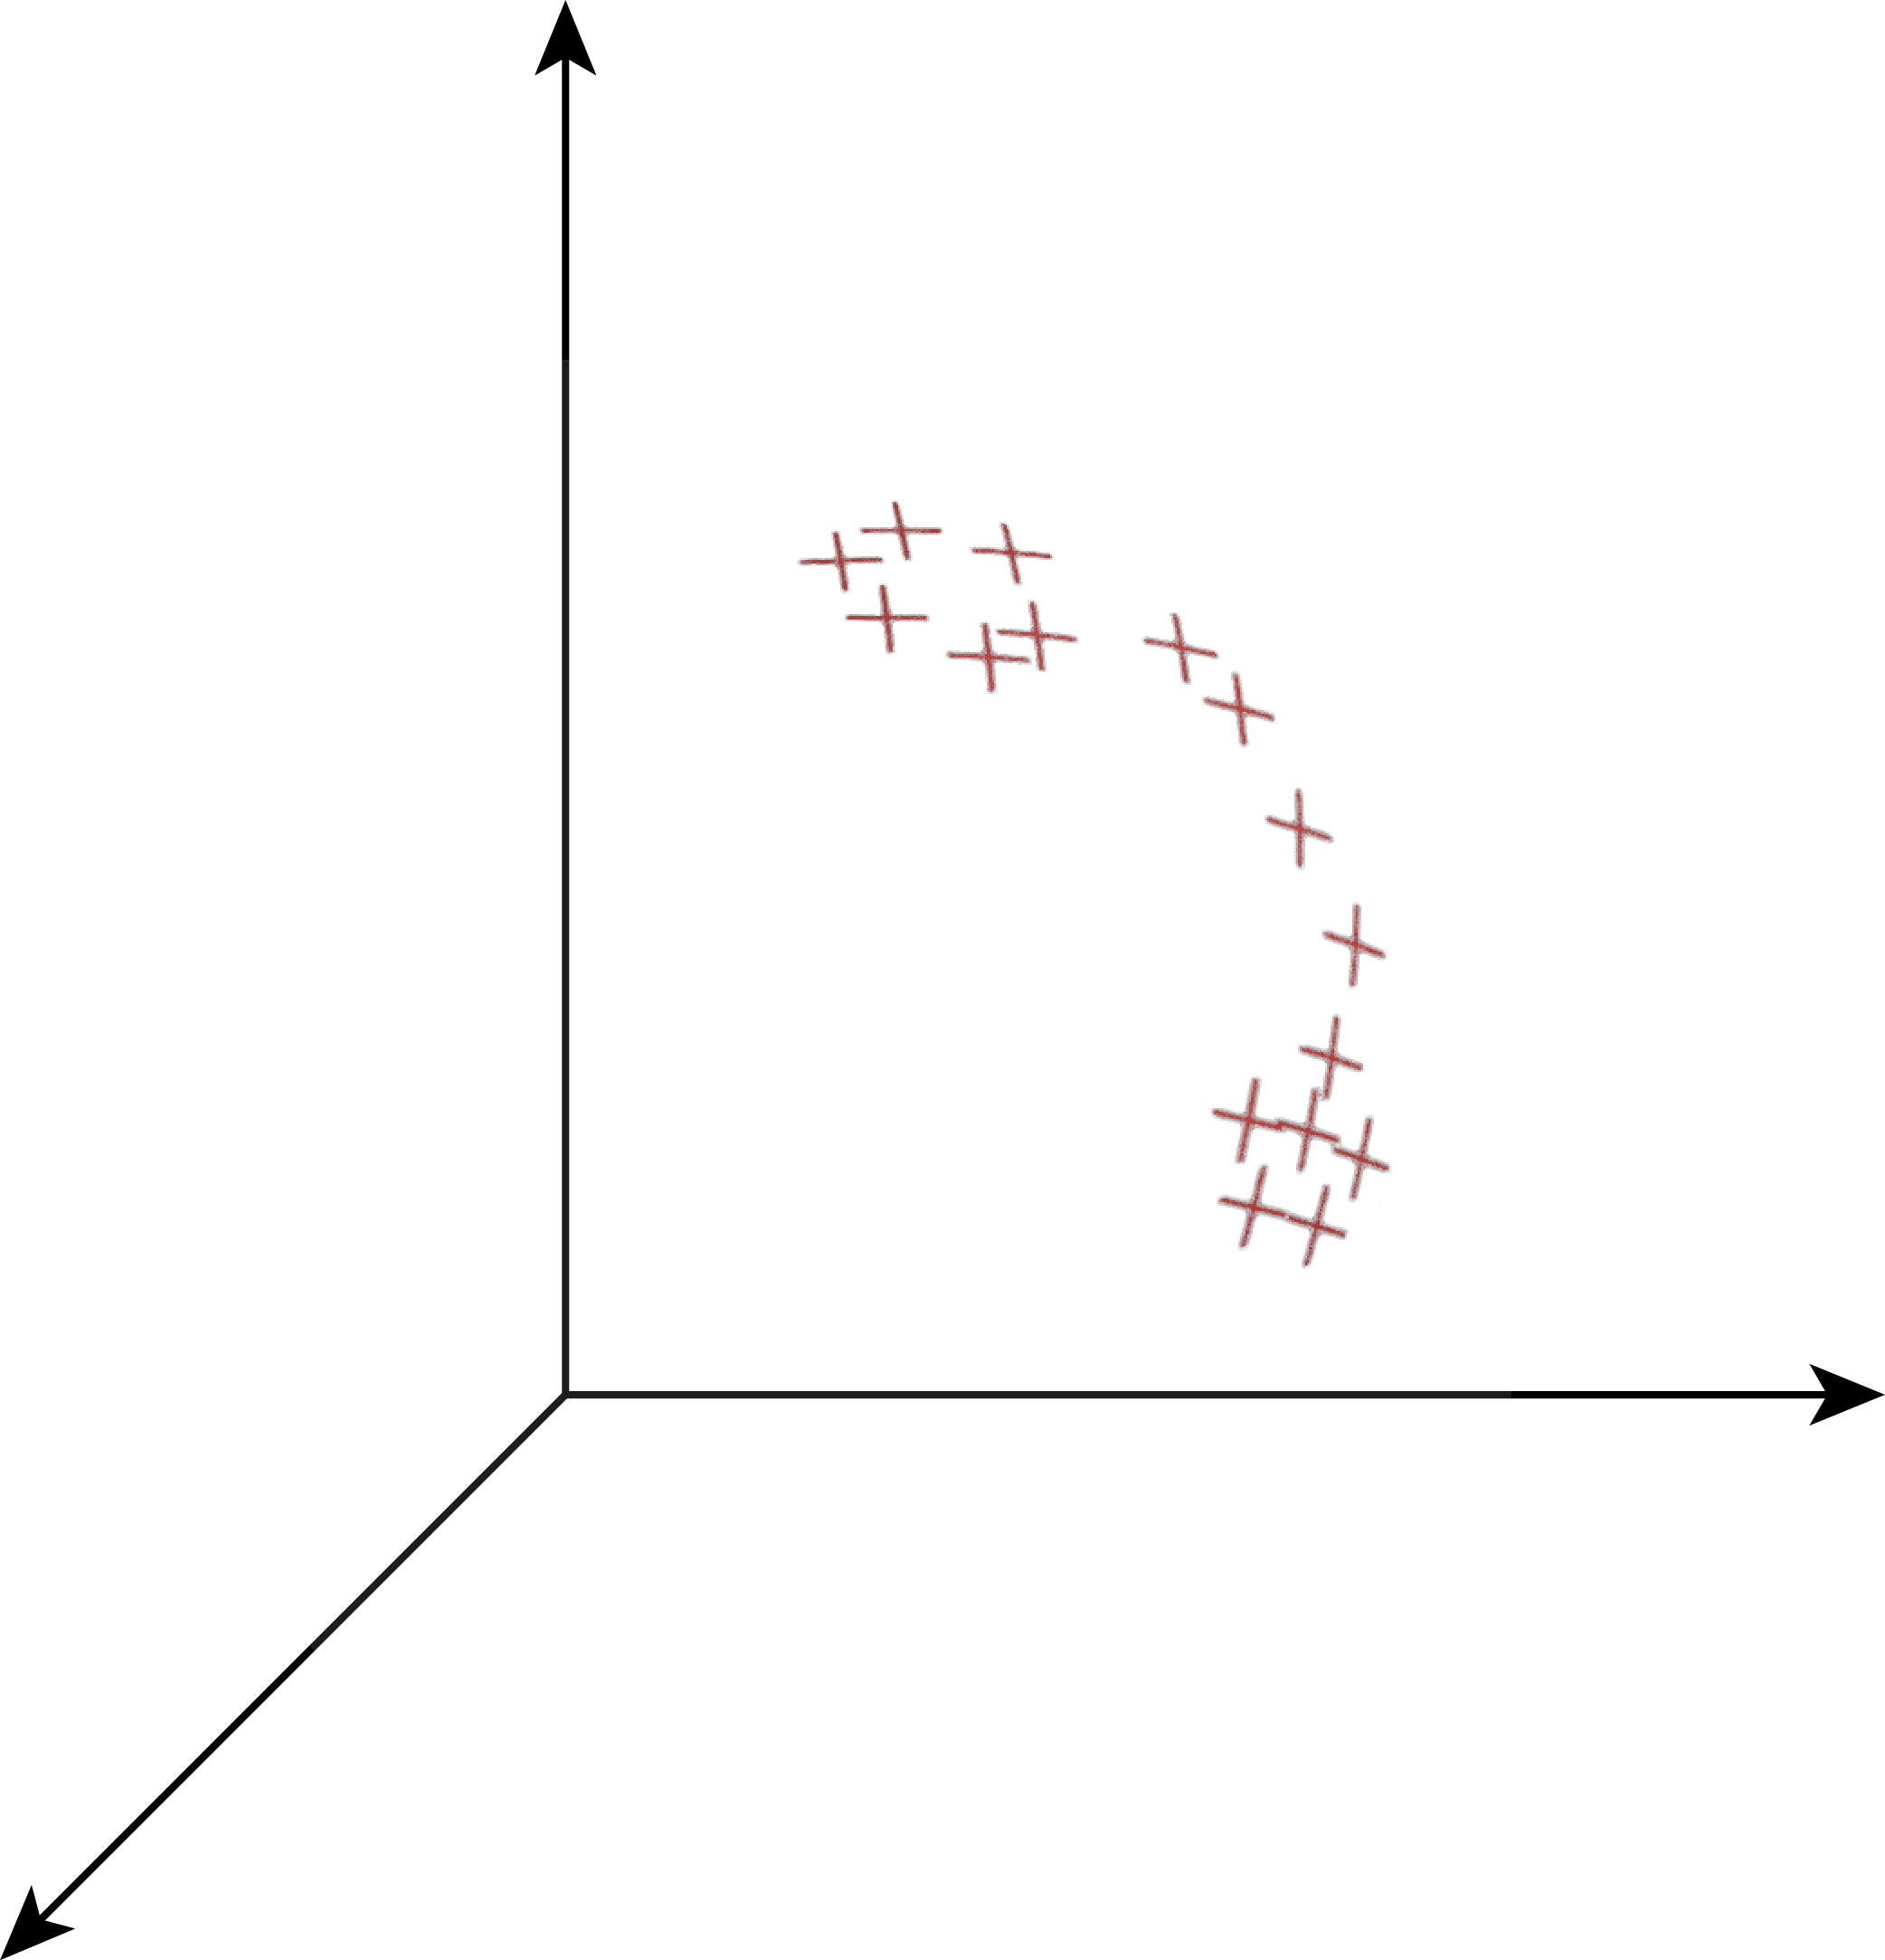
\includegraphics[width=\linewidth]{images/constraind_diffusion_rejection/intro_figure_euclidean@600x-100.jpg}
		\caption{$\R^3$}
		\label{fig:intro_figure_euclidean}
	\end{subfigure}
	\hfill
	\begin{subfigure}[b]{0.23\textwidth}
		\centering
		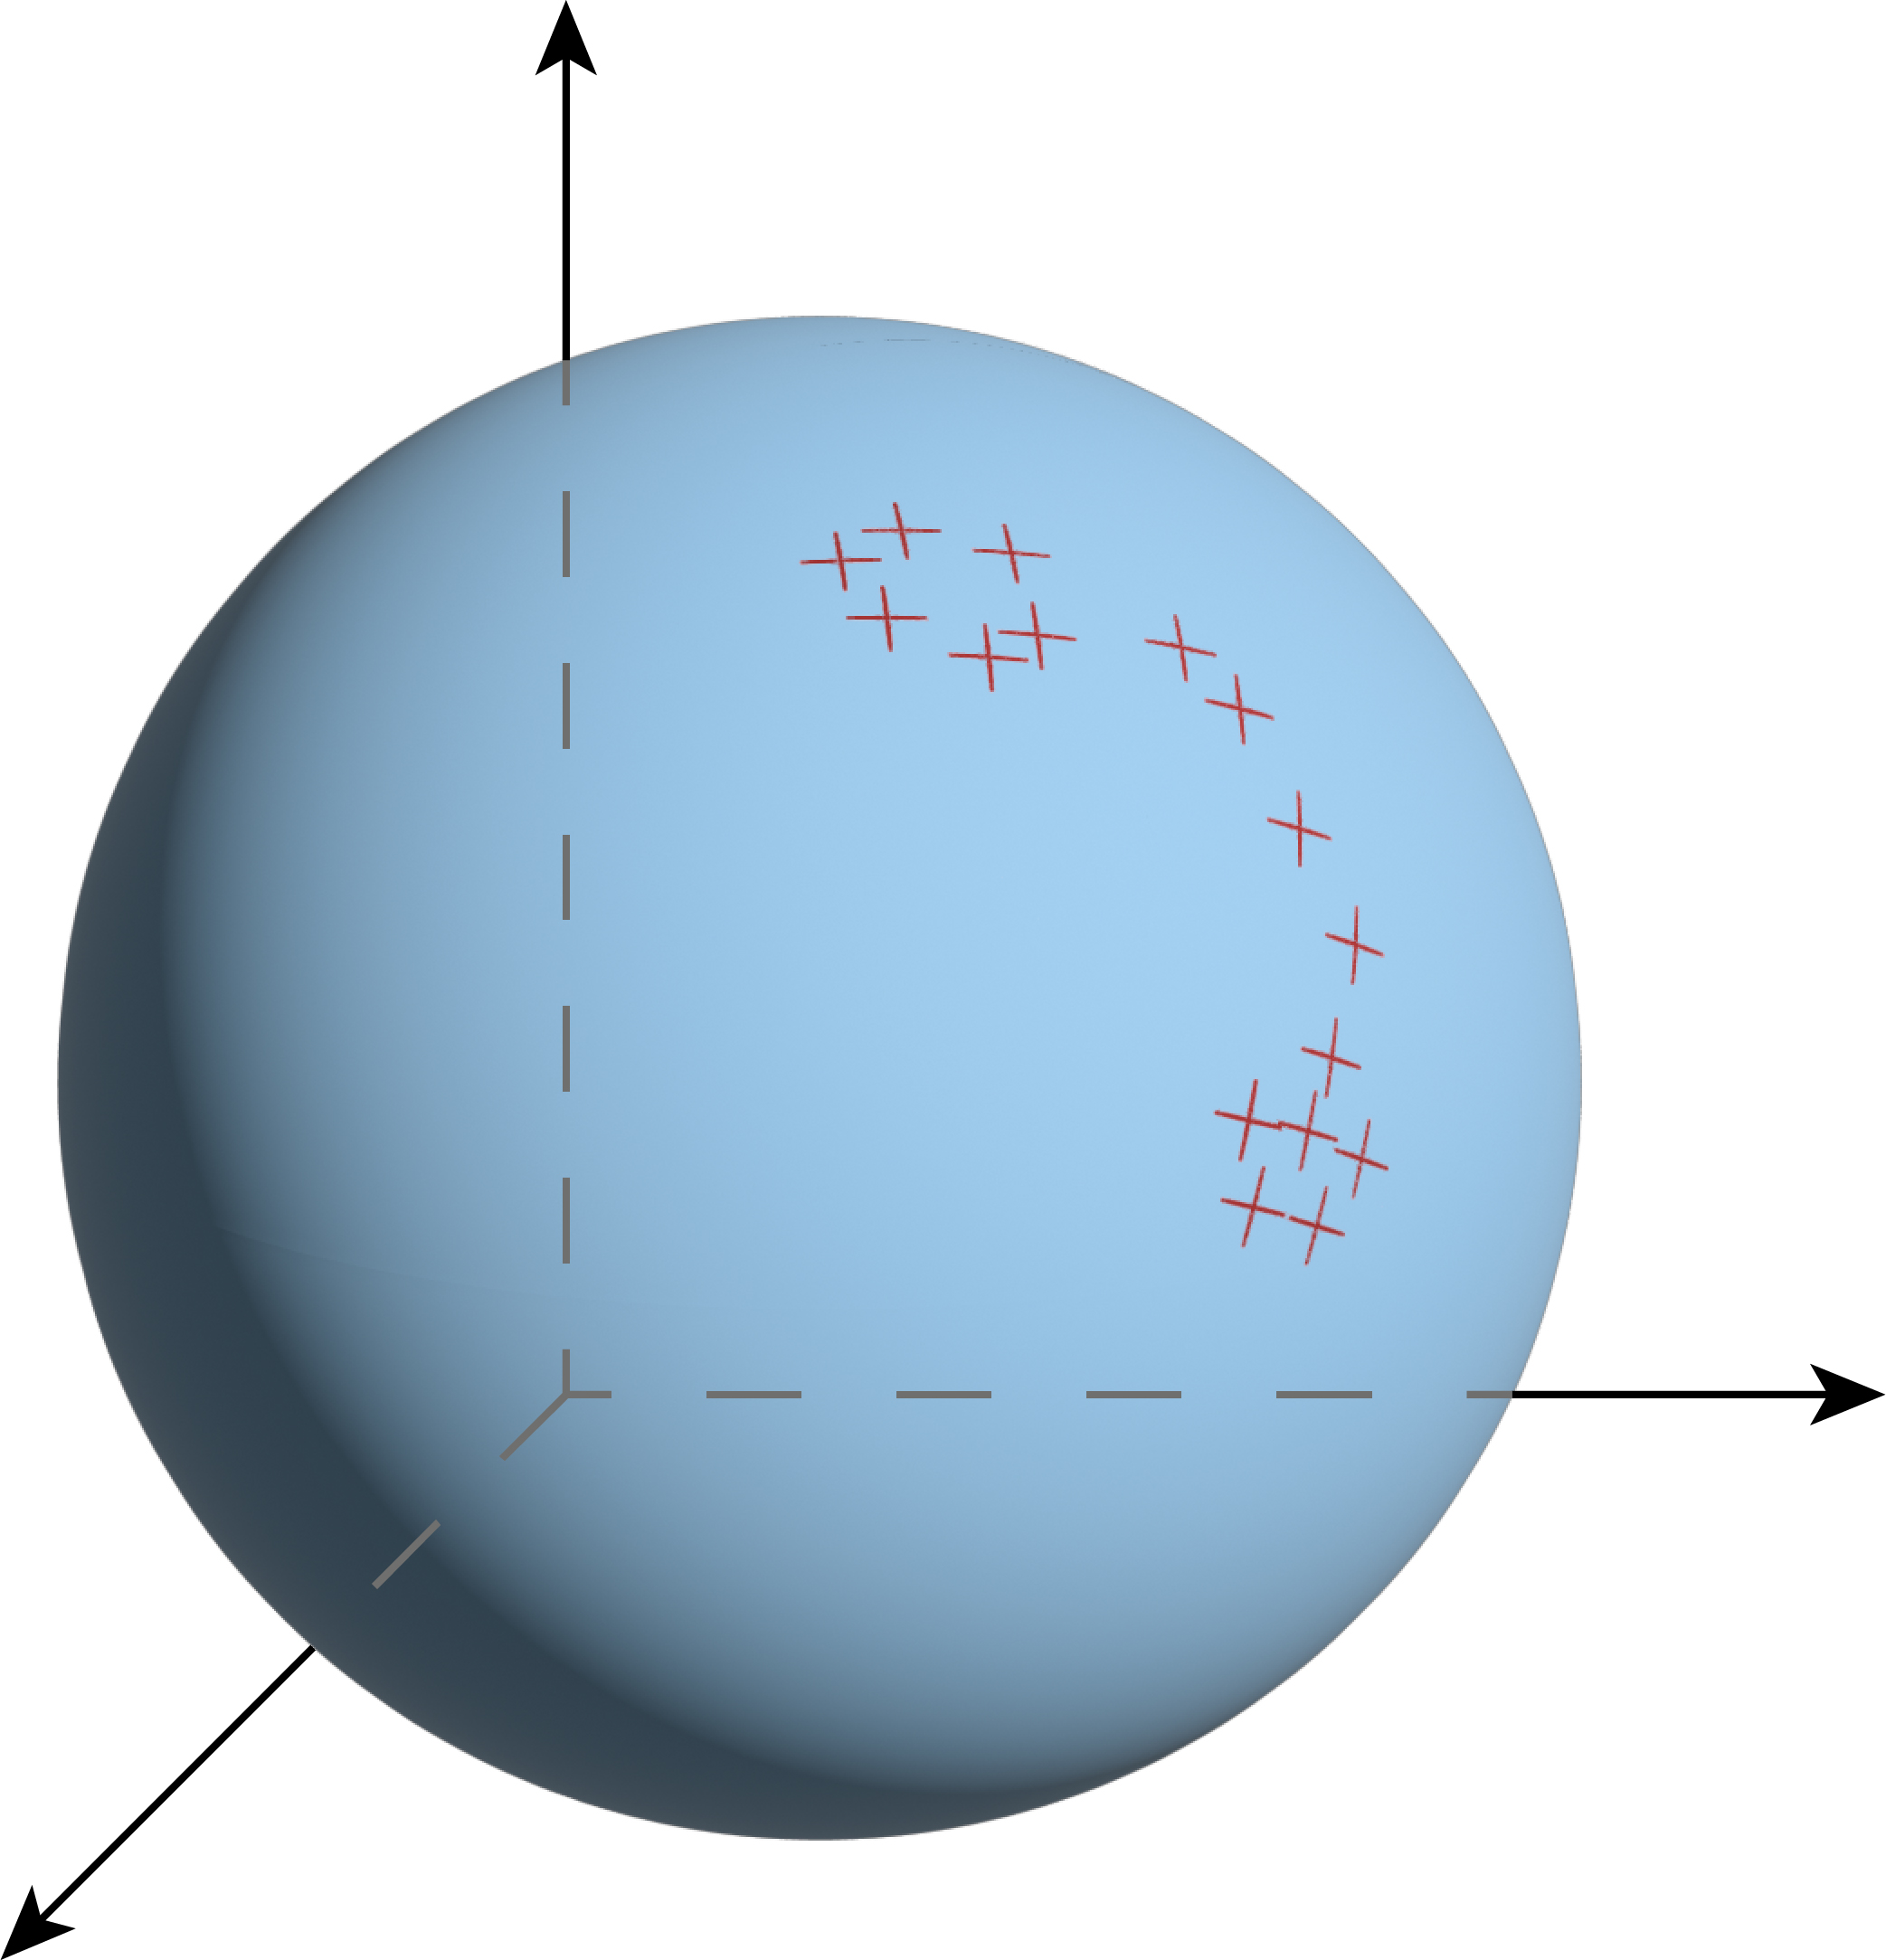
\includegraphics[width=\linewidth]{images/constraind_diffusion_rejection/intro_figure_manifold@600x-100.jpg}
		\caption{$\c{S}^2\subset\R^3$}
		\label{fig:intro_figure_manifold}
	\end{subfigure}
	\hfill
	\begin{subfigure}[b]{0.23\textwidth}
		\centering
		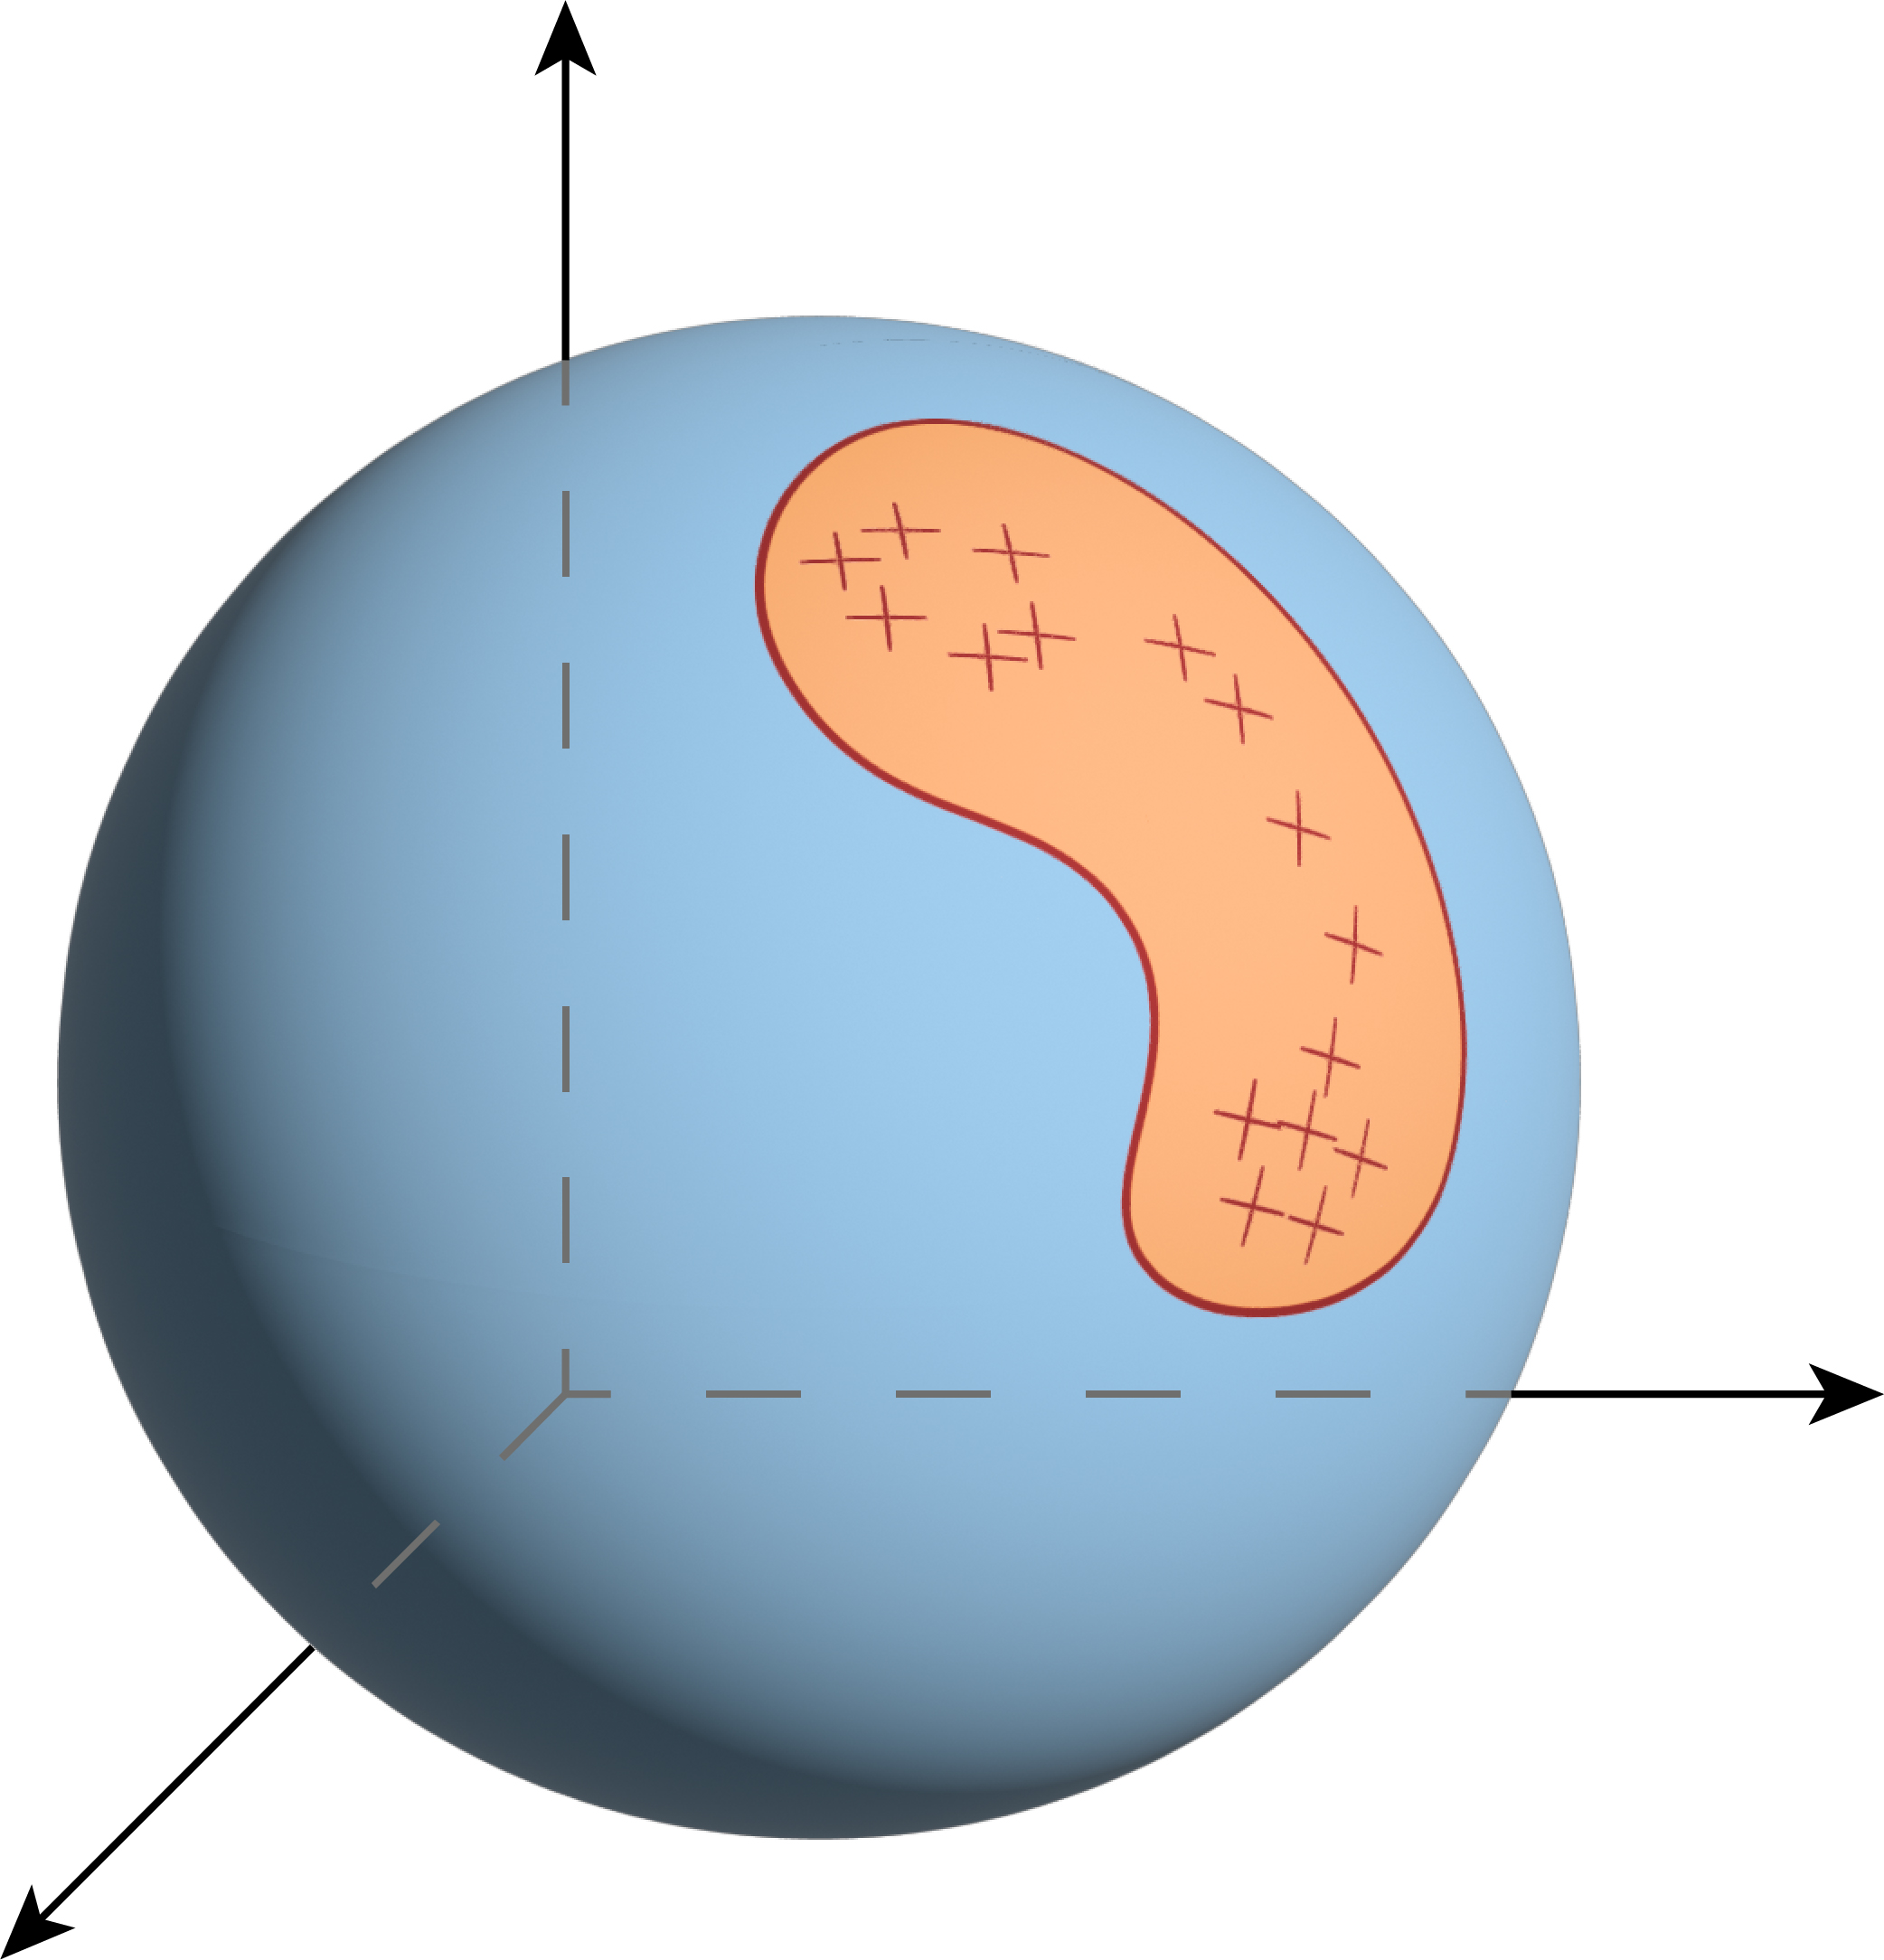
\includegraphics[width=\linewidth]{images/constraind_diffusion_rejection/intro_figure_constrained@600x-100.jpg}
		\caption{$\c{M}\subset\c{S}^2\subset\R^3$}
		\label{fig:intro_figure_constrained}
	\end{subfigure}
	\caption{When operating in data-scarce settings, it is often helpful to provide a model with as much prior information about the domain as possible.
		Consider a distribution over a subset $\c{M}$ of the unit sphere $\c{S}^2\subset\R^3$.
		While a Euclidean diffusion model can approximate the distribution in $\R^3$ (a), directly modelling it on $\c{S}^2$ can make learning significantly easier (b).
		Reducing the problem space even further by only constructing a diffusion model on $\c{M}$ can lead to even better performance (c).
	}
	\label{fig:intro_figure}
\end{figure}

\section{Background}

\paragraph{Riemannian manifolds.}
A Riemannian manifold is defined as a tuple $(\c{M}, \mathfrak{g})$ with $\c{M}$ a smooth manifold and $\mathfrak{g}$ a metric defining an inner product on tangent spaces.
In this work, we will use the exponential map $\exp_x: \mathrm{T}_x \c{M} \rightarrow \c{M}$, as well as the extension of the gradient $\nabla$, divergence $\dive$ and Laplace $\Delta$ operators to $\c{M}$.
All of these quantities can be defined in local coordinates in terms of the metric\footnote{if the connection chosen on the Riemannian manifold is the L\'{e}vi-Civita connection}.
The extension of the Laplace operator to $\c{M}$ is called the Laplace-Beltrami operator, also denoted $\Delta$ when there is no ambiguity.

Using $\Delta$, we can define a Brownian motion on $\c{M}$, denoted $(\v{B}_t)_{t \geq 0}$ and with density w.r.t.
the volume form of $\c{M}$ denoted $p_t$ for any $ t > 0$.
We refer to \textcite{lee2013smooth} for a thorough treatment of Riemannian manifolds and to \textcite{hsu2002stochastic} for details on stochastic analysis on manifolds.

In the following, we consider a manifold $\c{M}$ defined by \begin{equation} \label{eq:constrained_dupref} \c{M} = \cbrcolon{x \in \c{N}}{f_i(x) < 0 , \ i \in \c{I}}, \end{equation} where $(\c{N}, \mathfrak{g})$ is a Riemannian manifold, $\c{I}$ is an arbitrary finite indexing family and for any $i \in \c{I}$, $f_i\in \c{C}(\c{N}, \R)$.
Since $\c{I}$ is finite and $f_i$ continuous for any $i \in \c{I}$, $\c{M}$ is an open set of $\c{N}$ and inherits its metric $\mathfrak{g}$.
This captures simple Euclidean polytopes and complex constrained spaces like~\Cref{fig:intro_figure}.

\begin{figure}[t]
	\centering
	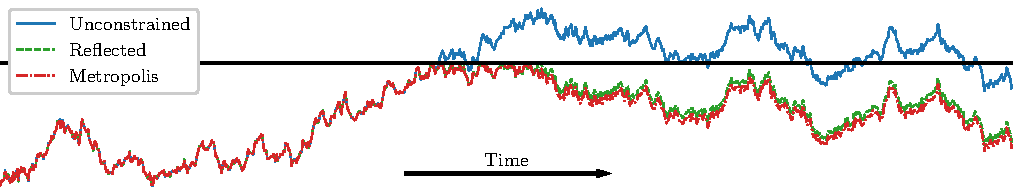
\includegraphics[width=\textwidth]{images/constraind_diffusion_rejection/rejection_vs_brownian_1d.pdf}

	\caption{Visual comparison of a discretisation of the unconstrained Brownian
		motion, two discretisations of the reflected Brownian motion: one based on
		a reflection scheme and the other based on our Metropolis sampler.
		The Metropolised trajectory is very close to that of the reflected one, while being significantly easier to implement and cheaper to compute.
	}
	\label{fig:1d_trajectories}
\end{figure}

\paragraph{Denoising diffusion models.}
\label{sec:sgm_dupref}
Denoising diffusion models \parencite{song2019generative,ho2020denoising,song2020score} work as follows: let $(\v{X}_{t})_{t \in \cbr{0,T}}$ be a \textit{noising process} that corrupts the original data distribution $p_0$.
We assume that $(\v{X}_t)_{t \geq 0}$ converges to $\mathrm{N}(0,\sigma^2\m{I})$, with $\sigma > 0$.
Several such processes exist, but in practice we consider the Ornstein-Uhlenbeck (OU) process, also referred as VP-SDE, which is defined by the following Stochastic Differential Equation (SDE) \begin{equation} \label{eq:ornstein_uhlenbeck_dupref} \mathrm{d} \v{X}_t = - \tfrac{1}{2}\v{X}_t \mathrm{d} t + \sigma \mathrm{d} \v{B}_t, \qquad \v{X}_0 \sim p_0.
\end{equation}
Under conditions on $p_0$, for any $T > 0$, $(\v{Y}_t)_{t \in \cbr{0,T}} = (\v{X}_{T-t})_{t \in \cbr{0,T}}$ is also the (weak) solution to a SDE \parencite{anderson1982reverse,haussmann1986time,cattiaux2021time} \begin{equation} \label{eq:time_reversal_dupref2} \textstyle \mathrm{d} \v{Y}_t = \{\tfrac{1}{2}\v{Y}_t + \sigma^2 \nabla \log p_{T-t}(\v{Y}_t)\} \mathrm{d} t + \sigma \mathrm{d} \v{B}_t, \ \v{Y}_0 \sim p_T, \end{equation} where $p_t$ denotes the density of $\v{X}_t$.

In practice, $\nabla \log p_t $ is approximated with a score network $(t,x) \mapsto s_\theta(t,x)$ trained by minimising either a denoising score matching ($\mathrm{dsm}$) loss or an implicit score matching ($\mathrm{ism}$) loss \parencite{vincent2011connection} \begin{equation} \label{eq:implicit_sm_dupref} \textstyle{ \ell(\theta) = \E_{t \sim \c{U}([0,T]), (\v{X}_0, \v{X}_t)}[ \lambda_t ( \frac{1}{2} \norm{ s_\theta(t, \v{X}_t) }^2 + \dive(s_\theta)(t, \v{X}_t))],} \end{equation} where $\lambda_t >0$.
For a flexible score network, the global minimiser $\theta^\star = \mathrm{argmin}_{\theta}\c{L}(\theta)$ satisfies $s_{\theta^\star}(t, \cdot)=\nabla \log p_t$.
\textcite{de2022riemannian}
and \textcite{huang2022riemannian} have extended denoising diffusion models to the
Riemannian setting.
The time-reversal formula \eqref{eq:time_reversal_dupref2} remains the same, replacing the Euclidean gradient with its Riemannian equivalent.
The \textrm{ism} loss can still be computed in that setting.
However, the samplers used in the Riemannian setting differ from the classical Euler-Maruyama discretisation used in the Euclidean framework.
\textcite{de2022riemannian}
use Geodesic Random Walks \parencite{jorgensen1975central}, which ensure that the
samples remain on the manifold at every step.
In this paper, we propose a sampler with similar properties in the case of \emph{constrained} manifolds.

\paragraph{Reflected SDE.}
We conclude this section by recalling the framework for studying reflected SDEs, which is introduced via the notion of the \emph{Skorokhod problem}.
For simplicity, we present this in the Euclidean space $\R^d$, but note that reflected processes can be defined on arbitrary smooth manifolds $\c{N}$.
In the case of the Brownian motion, a solution to the Skorokhod problem is a process of the form $(\bar{\v{B}}_t, \v{k}_t)_{t \geq 0}$.
Locally, $(\bar{\v{B}}_t)_{t \geq 0}$ can be seen as a regular Brownian motion $(\v{B}_t)_{t \geq 0}$ while $(\v{k}_t)_{t \geq 0}$ forces $(\bar{\v{B}}_t)_{t \geq 0}$ to remain in $\c{M}$.
Under mild additional regularity conditions on $\c{M}$ and $(\bar{\v{B}}_t, \v{k}_t)_{t \geq 0}$, see \cite{skorokhod1961stochastic}, $(\bar{\v{B}}_t, \v{k}_t)_{t \geq 0}$ is a solution to the \emph{Skorokhod problem} if for any $t \geq 0$ \begin{equation} \label{eq:rbm_dupref} \bar{\v{B}}_t = \bar{\v{B}}_0 + \v{B}_t - \v{k}_t \in \c{M}, \end{equation} $\textstyle{\abs{\v{k}}_t = \int_0^t \mathbf{1}_{\bar{\v{B}}_s \in \partial \c{M}} \mathrm{d} \abs{\v{k}}_s}$ and $\textstyle{\v{k}_t = \int_0^t \v{n}(\bar{\v{B}}_s) \mathrm{d} \abs{\v{k}}_s ,}$ where $(\abs{\v{k}}_t)_{t \geq 0}$ is the total variation of $(\v{k}_t)_{t \geq 0}$\footnote{In this case $(\v{k}_t)_{t \geq 0}$ is not regular enough, but if it were in the class $\c{C}^1$, its total variation would be given by $\int_0^t \abs{\partial_t \v{k}_t} \mathrm{d} s$ in the one-dimensional case.
}.

Let us provide some intuition on this definition.
When $(\bar{\v{B}}_t)_{t \geq 0}$ hits the boundary $\partial \c{M}$, $-\v{k}_t$ pushes the process back into $\c{M}$ along the inward normal $-\v{n}(\bar{\v{B}}_t)$, according to $\textstyle{\v{k}_t = \int_0^t \v{n}(\bar{\v{B}}_s) \mathrm{d} \abs{\v{k}}_s}$.
The condition $\textstyle{\abs{\v{k}}_t = \int_0^t \mathbf{1}_{\bar{\v{B}}_s \in \partial \c{M}} \mathrm{d} \abs{\v{k}}_s}$ is more technical and can be seen as imposing that $\v{k}_t$ remains constant so long as $(\bar{\v{B}}_t)_{t \geq 0}$ does not hit $\partial \c{M}$.
We refer to \cite{fishman2023diffusion} and \cite{lou2023reflected} for a more thorough introduction of these notions in the context of diffusion models.

\section{Diffusion models for constrained manifolds via Metropolis sampling}
\label{sec:methodology}

In~\Cref{sec:practical_constraints}, we highlight the practical limitations of existing constrained diffusion models and propose an alternative Metropolis sampling-based approach.
In \Cref{sec:theoretical_convergence}, we outline our proof that this process corresponds to a valid discretisation of the reflected Brownian motion, justifying its use in diffusion models.
An overview of the samplers we cover in this section is presented in~\Cref{tab:general_method_comparison}.

\subsection{Practical limitations of existing
	constrained diffusion models}
\label{sec:practical_constraints}

\begin{figure}[t]
	\centering
	\begin{subfigure}[t]{0.48\textwidth}
		\centering
		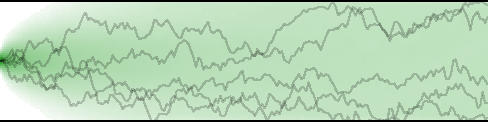
\includegraphics[width=\textwidth]{images/constraind_diffusion_rejection/reflected_density_no_text.pdf}
		\caption{Reflected Brownian motion}
	\end{subfigure}
	\hfill
	\begin{subfigure}[t]{0.48\textwidth}
		\centering
		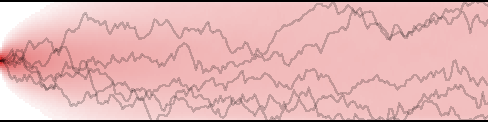
\includegraphics[width=\textwidth]{images/constraind_diffusion_rejection/rejection_density_no_text.pdf}
		\caption{Metropolised approximation of Brownian motion}
	\end{subfigure}
	\caption{Evolution of the density of the reflected Brownian motion and its Metropolis sampling-based approximation on the unit interval starting from a delta mass.}
	\label{fig:1d_densities}
\end{figure}

\paragraph{Barrier metrics.}
In the barrier approach, the constrained manifold is transformed into an unconstrained space via a barrier metric.
This metric is defined by $\nabla^2 \phi(x)$ with $\phi(x) = \sum_{i\in \c{I}} \phi_i(d(x, f_i))$ where \(d(x, f_i)\) is the minimum distance from the point \(x\) to the set defined by \(f_i(x) = 0\) and $\phi_i$ is a monotone decreasing function such that $\lim_{z \rightarrow 0} \phi_i(z) = \infty$ .
Under additional regularity assumptions, $\phi$ is called a \emph{barrier function} (see \cite{nesterov1994interior}).
This definition ensures that the barrier function induces a well-defined exponential map on the manifold, making the Riemannian diffusion model frameworks of \textcite{de2022riemannian} and \textcite{huang2022riemannian} applicable.
In practice, evaluating $\phi$ requires computing \(d(x, \partial \c{M})\) (and its derivatives), which can be prohibitively expensive.

Furthermore, since the exponential under the induced manifold is not easy to compute, the barrier methods in \cite{fishman2023diffusion} approximate it by projecting the exponential on the original manifold back into the constrained set, incurring additional bias and necessitating a projection, which can itself be computationally intractable, as we discuss in more detail below.

\paragraph{Reflected stochastic processes.}
\textcite{lou2023reflected} and \textcite{fishman2023diffusion} introduce diffusion models based on the
\emph{reflected Brownian motion} (RBM).
One possible discretisation of the reflected SDE is to \begin{enumerate*}[label=(\roman*)] \item consider a classical step of the Euler-Maruyama discretization (or the Geodesic Random Walk in the Riemannian setting) and \item reflect this step according to the boundary defined by $\partial \c{M}$.
\end{enumerate*}
To compute the reflection, one must check whether the step crosses the boundary.
If it does, the point of intersection needs to be calculated, the ray reflected at this point, and the step continued in the reflected direction.
This can require an arbitrarily large number of reflections depending on the step size, the geodesic on the manifold, and the geometry of the bounded region within the manifold.
We refer to \Cref{sec:reflected_discretisation} for the pseudocode of the reflection step and additional comments.

\begin{figure}{r}
	\begin{minipage}{0.42\textwidth}
		\begin{algorithm}[H]
			\caption{\emph{Metropolis approx. of RBM}}
			\label{alg:metropolis_approx}
			\begin{algorithmic}
				\Require \(p \in \c{M}\), \(\{f_i\}_{i \in \c{I}}\)
				\State Sample \(\v{v} \sim \mathrm{N}(0,\m{I}) \in \mathrm{T}_p\c{M}\)
				\State \(p' \gets \exp_{p}(\v{v})\)
				\If{\(f_i(p') < 0\ \forall\ i\)}
				\State \(p\gets p'\)
				\EndIf
				\Return \(p\)
			\end{algorithmic}
		\end{algorithm}
	\end{minipage}
\end{figure}
An alternative approach to discretising a reflected SDE is to replace the reflection with a projection, see \cite{slominski1994approximation} for instance.
However, the projection requires the most expensive part of the reflection algorithm: computing the intersection of the geodesic with the boundary.

\paragraph{Metropolis approximation.}
As outlined above, both of the existing approaches for constrained diffusion models require manifold- and constraint-specific implementations and become computationally intractable as the complexity and dimension of the modelled geometry increases.

This limits their practical usefulness even for relatively simple manifolds with well-defined exponential maps and linear inequality constraints (such as e.g. polytopes).

In the following, we introduce a method that aims to solve both of these problems.

The sampler we propose is similar to a classical Euler-Maruyama discretisation of the Brownian motion, except that, whenever a step would carry the Brownian motion outside of the constrained region, we reject it (see~\Cref{alg:metropolis_approx}).
This is a \emph{Metropolised} version of the usual discretisation and is almost trivial to implement compared to the existing barrier, reflection and projection methods.
Hence, this method enables the principled extension of diffusion models to arbitrarily constrained domains at virtually \emph{no added implementational complexity or computational expense}.

\begin{table}[t]
	\centering
	\caption{Comparing the requirements of different constrained diffusion models.}
	\label{tab:general_method_comparison}

	\adjustbox{width=\textwidth}{
		\small
		\begin{tabular}{lccc}
			\toprule
			\thead[l]{Sampling Method}                                  & \thead[c]{Set Indicator                   \\Function} & \thead[c]{Intersection\\Operator} & \thead[c]{Distance to\\Boundary} \\
			\midrule
			Barrier method \parencite{fishman2023diffusion}             & \cmark                  & \cmark & \cmark \\
			Reflected \parencite{fishman2023diffusion,lou2023reflected} & \cmark                  & \cmark & \xmark \\
			Projection sampler \parencite{lou2023reflected}             & \cmark                  & \cmark & \xmark \\
			Metropolis sampler (ours)                                   & \cmark                  & \xmark & \xmark \\
			\bottomrule
		\end{tabular}
	}
\end{table}

\subsection{Relating the Metropolis sampler to the reflected Brownian motion}
\label{sec:theoretical_convergence}

In this section, we prove that the proposed Metropolis sampling-based process (\Cref{alg:metropolis_approx}) corresponds to a valid discretization of the reflected process, justifying its use in diffusion models.
Here we focus on a concise presentation of the core concepts and the main results.
A full proof can be found in \Cref{sec:rejection-convergence}.
For simplicity, we restrict ourselves to the Euclidean setting.
All of our results require particular assumptions on $\c{M}$, which we discuss at the end of this section.
We begin with a definition of the Metropolis approximation of RBM.

\begin{definition}
	For any $\gamma >0$ and $k \in \N$, let $X_0^\gamma \in \c{M}$ and $X_{k+1}^\gamma = X_k^\gamma + \sqrt{\gamma} Z_k^\gamma$ if $X_k^\gamma + \sqrt{\gamma} Z_k^\gamma \in \c{M}$ and $X_k^\gamma$ otherwise.
	The sequence $(X_k^\gamma)_{k \in \N}$ is called the {Metropolis approximation of RBM}.
\end{definition}
For any $\gamma > 0$, we consider $(\v{X}_t^\gamma)_{t \geq 0}$, the linear interpolation of $(X^\gamma_k)_{k \in \N}$ such that for any $k \in \N$, $\v{X}_{k \gamma}^\gamma = X_k^\gamma$.
The following result is the main theoretical contribution of our paper.

\begin{theorem}
	\label{thm:weak_convergence_metropolis}
	Under assumptions on $\c{M}$, for any $T \geq 0$, $(\v{X}_t^\gamma)_{t \in \cbr{0,T}}$ weakly converges to the RBM $(\bar{\v{B}}_t)_{t \in \cbr{0,T}}$ as $\gamma \to 0$.

\end{theorem}

The rest of the section is devoted to a high level presentation of the proof of \Cref{thm:weak_convergence_metropolis}.
It is theoretically impractical to work directly with the Metropolis approximation of RBM.
Instead, we introduce an auxiliary process, show this converges to the RBM, and finally prove that the convergence of the auxiliary process implies the convergence of our Metropolis discretisation.

\begin{definition}
	For any $\gamma > 0$ and $k \in \N$, let $\hat{X}_0^\gamma = x \in \c{M}$ and $\hat{X}_{k+1}^\gamma = \hat{X}_k^\gamma + \sqrt{\gamma} Z_k^\gamma$ with $Z_k^\gamma$ a Gaussian random variable conditioned on $\hat{X}_k^\gamma + \sqrt{\gamma} Z_k^\gamma \in \c{M}$.
	The sequence $(\hat{X}_k^\gamma)_{k \in \N}$ is called the Rejection approximation of RBM.
\end{definition}

\begin{figure}
	\begin{minipage}{0.42\textwidth}
		\begin{algorithm}[H]
			\caption{\emph{Rejection approx. of RBM}}
			\label{alg:rejection_sampling}
			\begin{algorithmic}
				\Require \(p \in \c{M}\), \(\{f_i\}_{i \in \c{I}}\)
				\State Sample \(\v{v} \sim \mathrm{N}(0,\m{I}) \in \mathrm{T}_p\c{M}\)
				\State \(p' \gets \exp_{p}(\v{v})\)
				\While{\(f_i(p') \geq 0\ \text{for any}\ i\)}
				\State Sample \(\v{v} \sim \mathrm{Id}(0,1) \in \mathrm{T}_p\c{M}\)
				\State \(p' \gets \exp_{p}(\v{v})\)
				\EndWhile
				\Return \(p'\)
			\end{algorithmic}
		\end{algorithm}
	\end{minipage}
\end{figure}

We call this process \emph{Rejection approximation of RBM} since in practice, $Z_k^\gamma$ is sampled using rejection sampling, see~\Cref{alg:rejection_sampling}.
For any $\gamma > 0$, we also consider $(\hat{\v{X}}_t^\gamma)_{t \geq 0}$, the linear interpolation of $(\hat{X}^\gamma_k)_{k \in \N}$ such that for any $k \in \N$, $\hat{\v{X}}_{k \gamma}^\gamma = \hat{X}_k^\gamma$.
In~\Cref{sec:rejection-convergence}, we prove the following result.

\begin{theorem}
	\label{thm:weak_convergence_rejection}
	Under assumptions on $\c{M}$, for any $T \geq 0$, $(\hat{\v{X}}_t^\gamma)_{t \in \cbr{0,T}}$ weakly converges to the Reflected Brownian Motion $(\bar{\v{B}}_t)_{t \in \cbr{0,T}}$ as $\gamma \to 0$.

\end{theorem}

\begin{proof}
	Here we give some elements of the proof.
	Details and full derivations are postponed to \Cref{sec:rejection-convergence}.
	Our approach is based on the invariance principle of \cite{stroock1971diffusion}.
	More precisely, we show that we can compute an equivalent `drift' and `diffusion matrix' for the discretised process and that, as $\gamma \to 0$, the drift converges to zero and the diffusion matrix converges to $\m{I}$.
	In the Euclidean setting, this result, accompanied by mild regularity and growth assumptions, ensures that the discretization weakly converges to the original SDE.
	However, the case with boundary is much more complicated, primarily because the approximate drift might explode near the boundary, thus we need to verify exactly how the drift behaves as $\gamma \to 0$ and as the process approaches the boundary.
	We show that the \emph{normalised} drift converges to the inward normal near the boundary.
	This ensures that \begin{enumerate*}[label=(\alph*)] \item in the interior of $\c{M}$ the drift converges to zero, i.e.~locally in the interior of $\c{M}$ the Brownian motion and the Reflected Brownian Motion coincide, \item on the boundary, the drift pushes the samples inside the manifold according to the inward normal, mimicking $(\v{k}_t)_{t \geq 0}$ in \eqref{eq:rbm_dupref}.
	\end{enumerate*}
	Finally, with results from \cite{stroock1971diffusion} and \cite{kang2017submartingale}, we show the convergence to the RBM.

\end{proof}

Our next step is to show that the approximate drift and diffusion matrix of the Metropolised process are upper and lower bounded by their counterparts in the rejection process.
While the upper-bound is easy to derive, the lower-bound requires the following result.

\begin{proposition}
	\label{lemma:lower_bound_prob_main}
	Under assumptions on $\c{M}$, $\forall \; \varepsilon > 0$, $\exists \; \bar{\gamma} >0$ such that for any $\gamma \in \del{0, \bar{\gamma}}$ and for any $x \in \c{M}$, $\gamma \in \del{0, \bar{\gamma}}$ and $Z \sim \mathrm{N}(0, \m{I})$ we have $\mathbb{P}(x + \sqrt{\gamma} Z \in \c{M}) \geq 1/2-\varepsilon$, with $Z \sim \mathrm{N}(0, \m{I})$.
\end{proposition}

\Cref{lemma:lower_bound_prob_main} tells us that \emph{locally} the boundary
looks like a half-space when integrating w.r.t. a Gaussian measure.
A corollary is that, for $\gamma > 0$ small enough and for any $k \in \N$, the probability that $X_{k+1}^\gamma = X_k^\gamma$ is upper bounded \emph{uniformly} w.r.t.
$X_k^\gamma \in \c{M}$.
The proof of \Cref{lemma:lower_bound_prob_main} uses \Cref{thm:tubul-neighb} in~\Cref{sec:rejection-convergence}, whose proof relies on the concept of \emph{tubular neighborhoods} \parencite{lee2013smooth}.

Having established the lower and upper bound, we can conclude the proof by noting that the approximate drift and the diffusion matrix in the rejection and Metropolis case coincide as $\gamma \to 0$.
This is enough to apply the same results as before, giving the desired convergence.

\paragraph{Assumptions on $\c{M}$.}
Before concluding this section, we detail the assumptions we make on $\c{M}$.
For \Cref{thm:weak_convergence_metropolis} to hold, we assume that $\c{M} = \cbrcolon{x \in \R^d}{\Phi(x) > 0}$ is bounded, with $\Phi \in \c{C}^2(\R^d, \R)$ concave.
We have that $\partial \c{M} = \cbrcolon{x \in \R^d}{\Phi(x) = 0}$.
In addition, we assume that for any $x \in \partial \c{M}$, $\norm{\nabla \Phi(x)} = 1$.
These assumptions match those \cite{stroock1971diffusion} use for their study of the existence of solutions to the RBM.
While it seems possible to relax the \emph{global} existence of $\Phi$ to a \emph{local} one, the regularity assumption of the domain is key.
This regularity is essential to establish \Cref{lemma:lower_bound_prob_main} and the associated geometrical result on tubular neighborhoods.
We also emphasize that the smoothness of the domain is central in the results of \cite{kang2017submartingale} on the equivalence of two definitions of RBMs which we rely on.

\section{Related work on approximations of reflected SDEs}

Several schemes have been introduced to approximately sample from reflected Stochastic Differential Equations.
They can be interpreted as modifications of classical Euler-Maruyama schemes used to discretise SDEs without boundary.
One of the most common approaches is to use the Euler-Maruyama discretisation and project the solution onto the boundary if it escapes from the domain $\c{M}$.
In this case, mean-square error rates of order \emph{almost} $1/2$ have been proven under various conditions \parencite{liu1995discretization,chitashvili1981strong,pettersson1995approximations,slominski1994approximation}.
Concretely this means that $\E[\| \bar{\v{B}}_{t} - X_{n}^{t/n}\|^2] = O(n^{-1+\varepsilon})$ with $\varepsilon>0$ arbitrary small and where $(X_k^\gamma)_{k \in \N}$ is the projection scheme.

The rate $1/2$ is tight \parencite{pacchiarotti1998numerical}.
It is possible to use the Euler-Peano method to get slight improvements for a mean-square error rate of order of $1/2$, but this is impractical as it assumes that one can solve a (simplified) Skorokhod problem, which is usually intractable.

\textcite{liu1993numerical} introduced a \emph{penalised}
method which pushes the solution away from the boundary and shows a mean-square error
of order $1/4$, see also \cite{pettersson1997penalization}.
Weak errors of order $1$ have been obtained in \cite{bossy2004symmetrized} and \cite{gobet2001euler} by introducing a reflection component in the discretisation or using some local approximation of the domain to a half-space.
We refer to \cite{pilipenko2014introduction} for an introduction to the discretisation of reflected SDEs.
Closer to our work, \cite{burdzy2008discrete} consider three different methods to approximate reflected Brownian motions on general domains (two based on discrete methods and one based on killed diffusions).
Only qualitative results are provided.
To the best of our knowledge, no previous work in the probability literature has investigated the \emph{Metropolised} scheme we propose.

Our Metropolis scheme is also related to the ball walk \parencite{applegate1991sampling}, which replaces the Gaussian random variable with a uniform over the ball (or the Dikin ellipsoid).
\textcite{applegate1991sampling} and \cite{lovasz2007geometry} have
studied the asymptotic convergence rate of the ball walk, but, to the best of our
knowledge, its limiting behaviour when the step size goes to zero has not been
investigated.

\section{Experimental results}

\begin{figure}[t]
	\centering
	\begin{subfigure}[t]{0.23\textwidth}
		\centering
		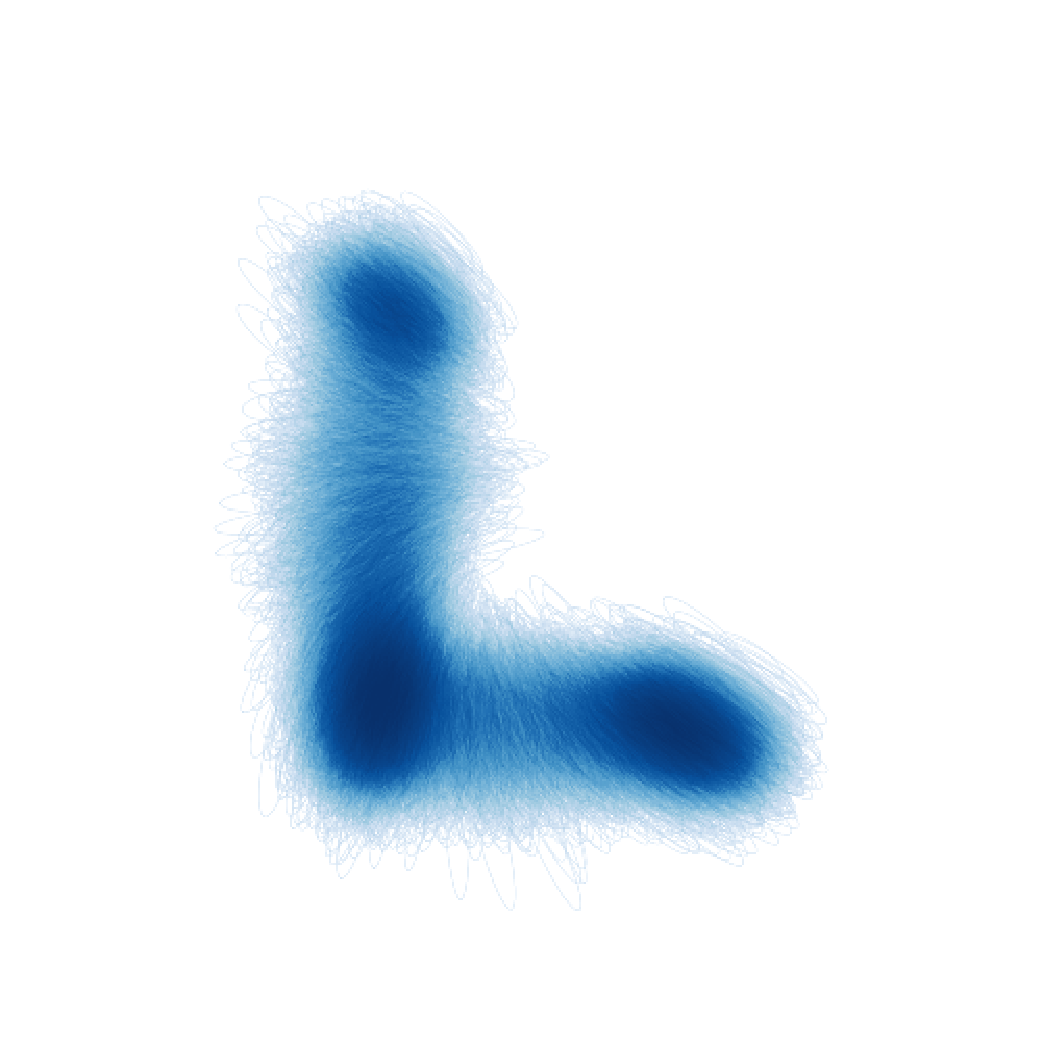
\includegraphics[width=\linewidth]{images/constraind_diffusion_rejection/spd_main_data.pdf}
		\caption{Data distribution.}
		\label{fig:robotic_arm_data}
	\end{subfigure}
	\hfill
	\begin{subfigure}[t]{0.23\textwidth}
		\centering
		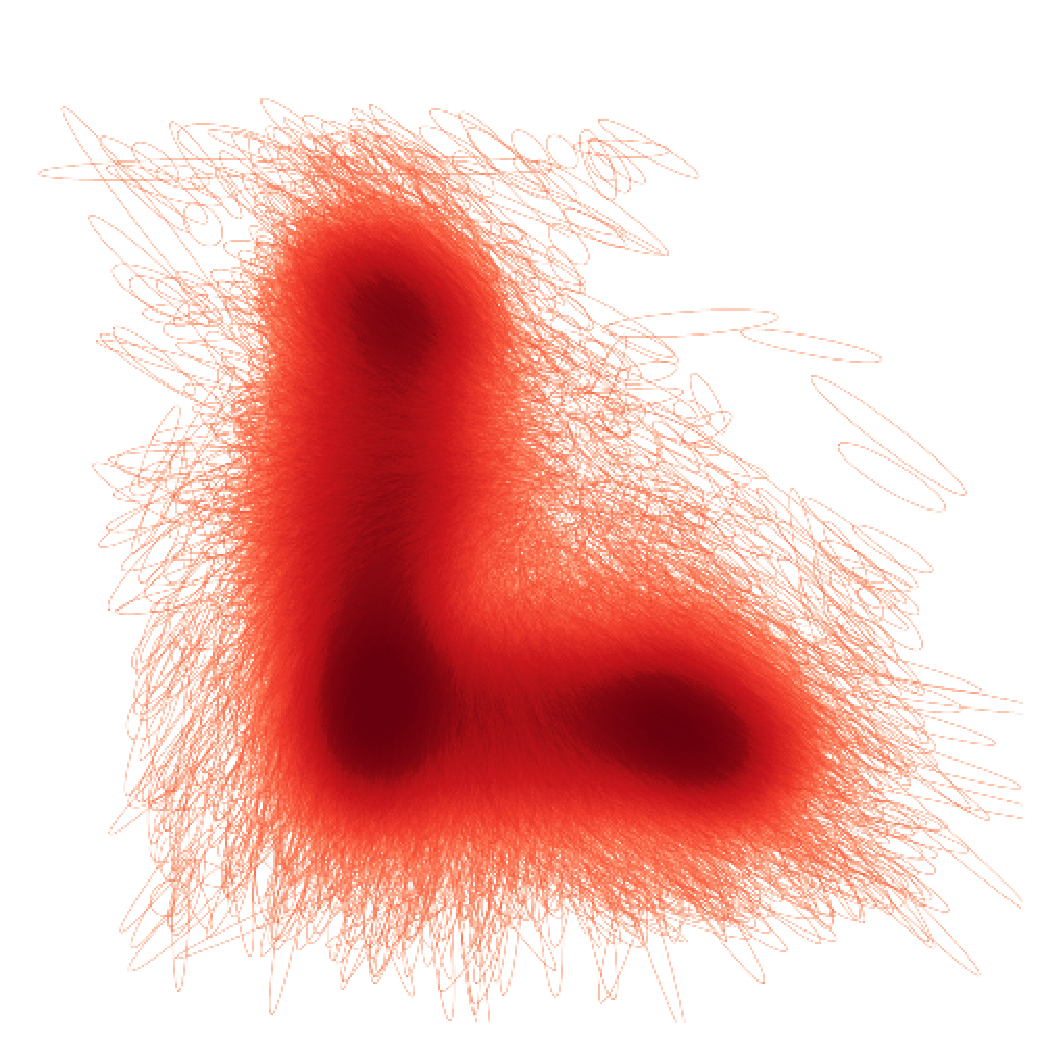
\includegraphics[width=\linewidth]{images/constraind_diffusion_rejection/spd_main_rejection.pdf}
		\caption{Metropolis samples.}
		\label{fig:robotic_arm_rejection}
	\end{subfigure}
	\hfill
	\begin{subfigure}[t]{0.23\textwidth}
		\centering
		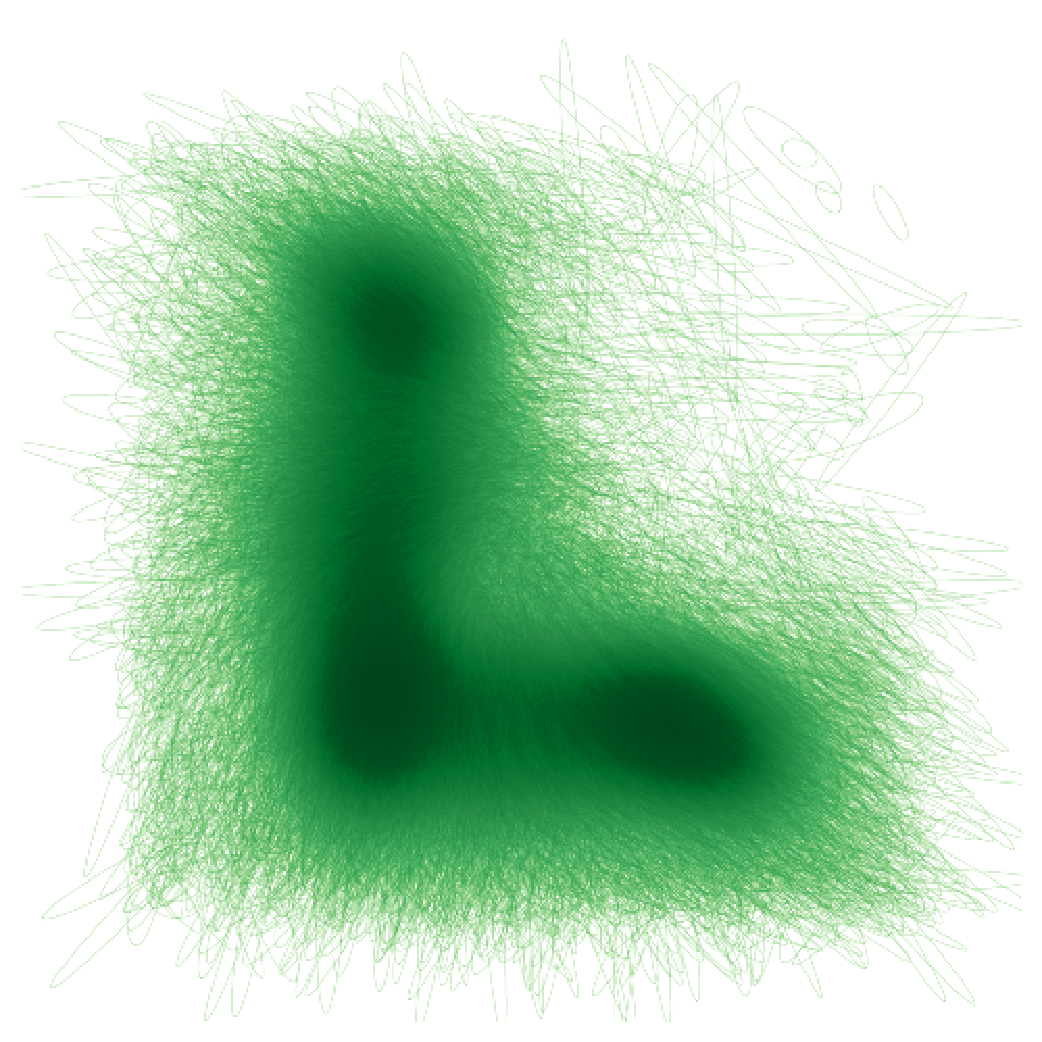
\includegraphics[width=\linewidth]{images/constraind_diffusion_rejection/spd_main_reflected.pdf}
		\caption{Reflected samples.}
		\label{fig:robotic_arm_reflected}
	\end{subfigure}
	\hfill
	\begin{subfigure}[t]{0.23\textwidth}
		\centering
		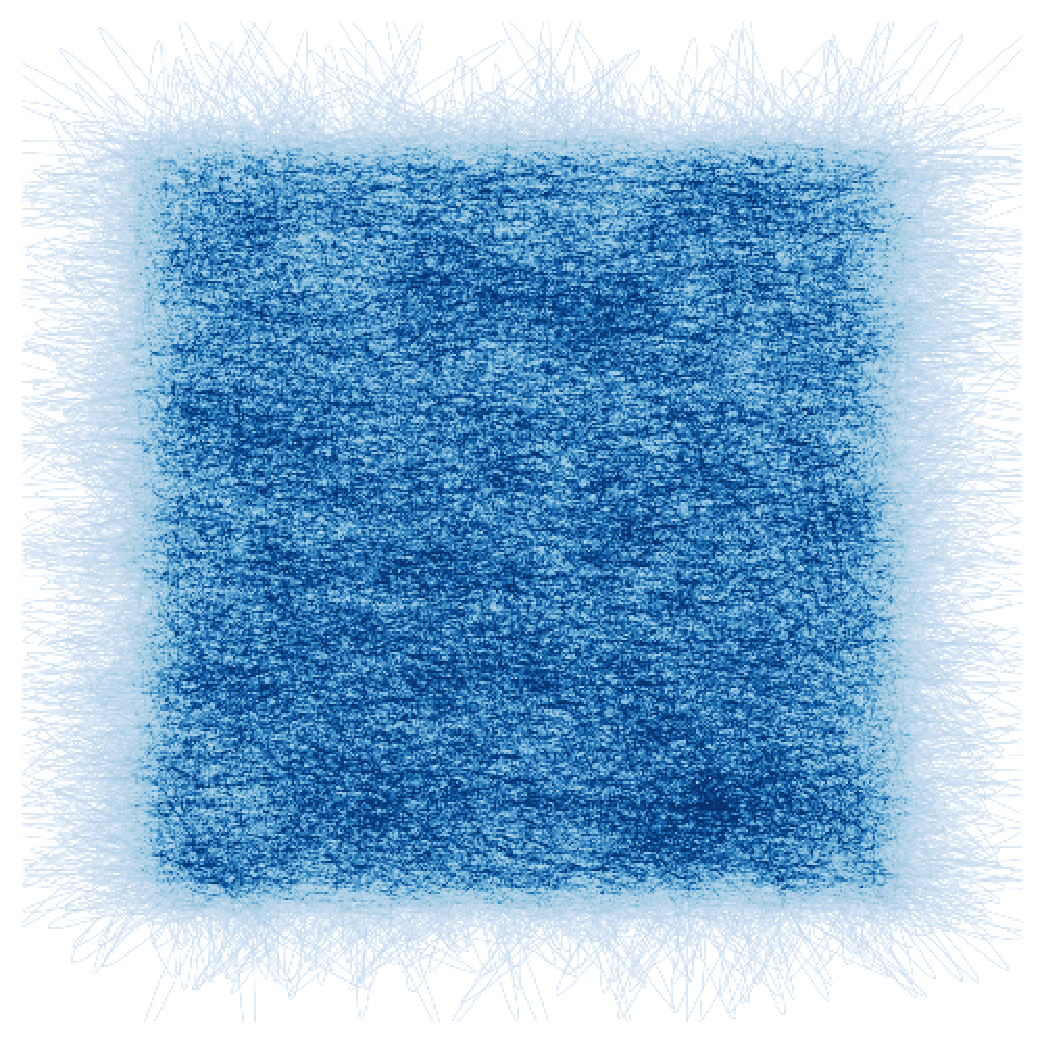
\includegraphics[width=\linewidth]{images/constraind_diffusion_rejection/spd_main_uniform.pdf}
		\caption{Uniform distribution.}
		\label{fig:robotic_arm_uniform}
	\end{subfigure}
	\caption{A qualitative visual comparison of $10^6$ samples from the data distribution, our Metropolis diffusion model, a reflected diffusion model and the uniform distribution for the constrained configurational modelling of robotic arms on \(\c{S}_{++}^2\times \R^2\).}
	\label{fig:robotic_arm}
\end{figure}

To demonstrate the practical utility and empirical performance of the proposed Metropolis diffusion models, we conduct a comprehensive evaluation on a range of synthetic and real-world tasks.
In~\Cref{sec:exp_synthetic_tasks}, we assess the scalability of our method by applying it to synthetic distributions on hypercubes and simplices of increasing dimensionality.
In~\Cref{sec:exp_arms_and_backbones}, we extend the evaluation to real-world tasks on manifolds with convex constraints by applying our method to the robotics and protein design datasets presented in \cite{fishman2023diffusion}.

In~\Cref{sec:exp_wildfires}, we additionally demonstrate that our method extends to constrained manifolds with highly \emph{non-convex} boundaries---a setting that is intractable with existing approaches.
As we found---in line with \cite{fishman2023diffusion}---that log-barrier diffusion models perform strictly worse than reflected approaches across all experimental settings, we focus on a more detailed comparison with the latter here and postpone additional empirical results to~\Cref{sec:app_exp_barrier_results}.

For all experiments, we use a simple 6 layer MLP with sine activations and a score rescaling function to ensure that the score reaches zero at the boundary, scaling linearly into the interior of the constrained set as in \cite{liu2022estimating} and \cite{fishman2023diffusion}.
We set $T=1$, $\beta_0=\num{1e-3}$ and tune $\beta_1$ to ensure that the forward process reaches the invariant distribution with a linear $\beta$-schedule.
We use a learning rate of \num{2e-4} with a cosine learning rate schedule and an $\mathrm{ism}$ loss with a modified loss weighting function of $(1 + t)$, a batch size of 256 and 8 repeats per batch.
All models were trained on a single NVIDIA GeForce GTX 1080 GPU.
Additional details are provided in~\Cref{sec:app_implementational_details}.

\subsection{Synthetic distributions on simple polytopes}
\label{sec:exp_synthetic_tasks}

\begin{table}
	\caption{
		Log-likelihood ($\uparrow$) of a held-out test set from a synthetic bimodal distribution over convex subsets of $\R^d$ bounded by the hypercube \([-1,1]^d\) and unit simplex \(\Delta^d\).
		Means and standard deviations are computed over 3 different runs.
		Training time in hours is listed in parentheses.
	}
	\label{tab:synthetic_polytope_dupref}
	\centering

	\begin{tabular}{clll}
		\toprule
		Constraint & \(d\) & {Reflected \emph{(hours)}}    & {Metropolis \emph{(hours)}}              \\
		\midrule
		\multirow{3}{*}{$[-1,1]^d$}
		           & 2     & $2.25\pm{.01}$ \emph{(8.95)}  & $\mathbf{2.32\pm{.05}}$ \emph{(0.72)}    \\
		           & 3     & $3.77\pm{.13}$ \emph{(8.97)}  & $\mathbf{4.15\pm{.15}}$ \emph{(0.71)}    \\
		           & 10    & $7.42\pm{.77}$ \emph{(10.15)} & $\mathbf{10.80 \pm{.34 }}$ \emph{(0.90)} \\
		\midrule
		\multirow{3}{*}{$\Delta^d$}
		           & 2     & $1.01 \pm{.01}$ \emph{(9.17)} & $\mathbf{1.06\pm{.02}}$ \emph{(0.82)}    \\
		           & 3     & $2.64\pm{.01}$ \emph{(9.43)}  & $\mathbf{3.23\pm{.17}}$  \emph{(0.78)}   \\
		           & 10    & $7.00\pm{.13}$ \emph{(10.53)} & $\mathbf{7.81\pm{.20}}$ \emph{(0.97)}    \\
		\bottomrule
	\end{tabular}
\end{table}

In this section, we investigate the scalability of the proposed Metropolis diffusion models by applying them to synthetic bimodal distributions over the \(d\)-dimensional hypercube \([-1, 1]^d\) and unit simplex \(\Delta^{d}\).
A quantitative comparison of the log-likelihood of a held-out test set is presented in~\Cref{tab:synthetic_polytope_dupref}, while a visual comparison is postponed to~\Cref{sec:app_exp_synthetic_tasks}.

We find that our Metropolis models outperform reflected approaches across all dimensions and constraint geometries by a substantial and statistically significant margin while training in one tenth of the time.

The degree of improvement seems to scale with the dimensionality of the problem: the larger the dimension of the experiment, the larger the gain in performance from using our proposed Metropolis scheme.

\subsection{Modelling proteins and robotic arms under convex constraints}
\label{sec:exp_arms_and_backbones}

In addition to illustrating our method's scalability on high-dimensional synthetic tasks, we follow the experimental setup from \cite{fishman2023diffusion} to additionally demonstrate its practical utility and favourable empirical performance on two real-world problems from robotics and protein design.

\paragraph{Constrained configurational modelling of robotic arms.}
The problem of modelling the configurations and trajectories of a robotic arm can be formulated as learning a distribution over the locations and manipulability ellipsoids of its joints, parameterised on \(\R^d\times\c{S}_{++}^d\), where \(\c{S}_{++}^d\) is the manifold of symmetric positive-definite (SPD) \(d\times d\) matrices \parencite{yoshikawa1985manipulability, jaquier2021geometry}.
For practical robotics applications, it may be desirable to restrict the maximal velocity with which a robotic arm can move or the maximum force it can exert.
This manifests in a trace constraint $C>0$ on \(\c{S}_{++}^d\), resulting in a constrained manifold \(\{M\in\c{S}_{++}^d:\sum_{i=1}^dM_{ii} < C\}\).
Following \cite{fishman2023diffusion}, we parametrise this constraint via the Cholesky decomposition \parencite{lin2019riemannian} and use the resulting setup to model the dataset presented in \cite{jaquier2021geometry}.

\begin{figure}[t]
	\centering
	\begin{subfigure}[t]{0.23\textwidth}
		\centering
		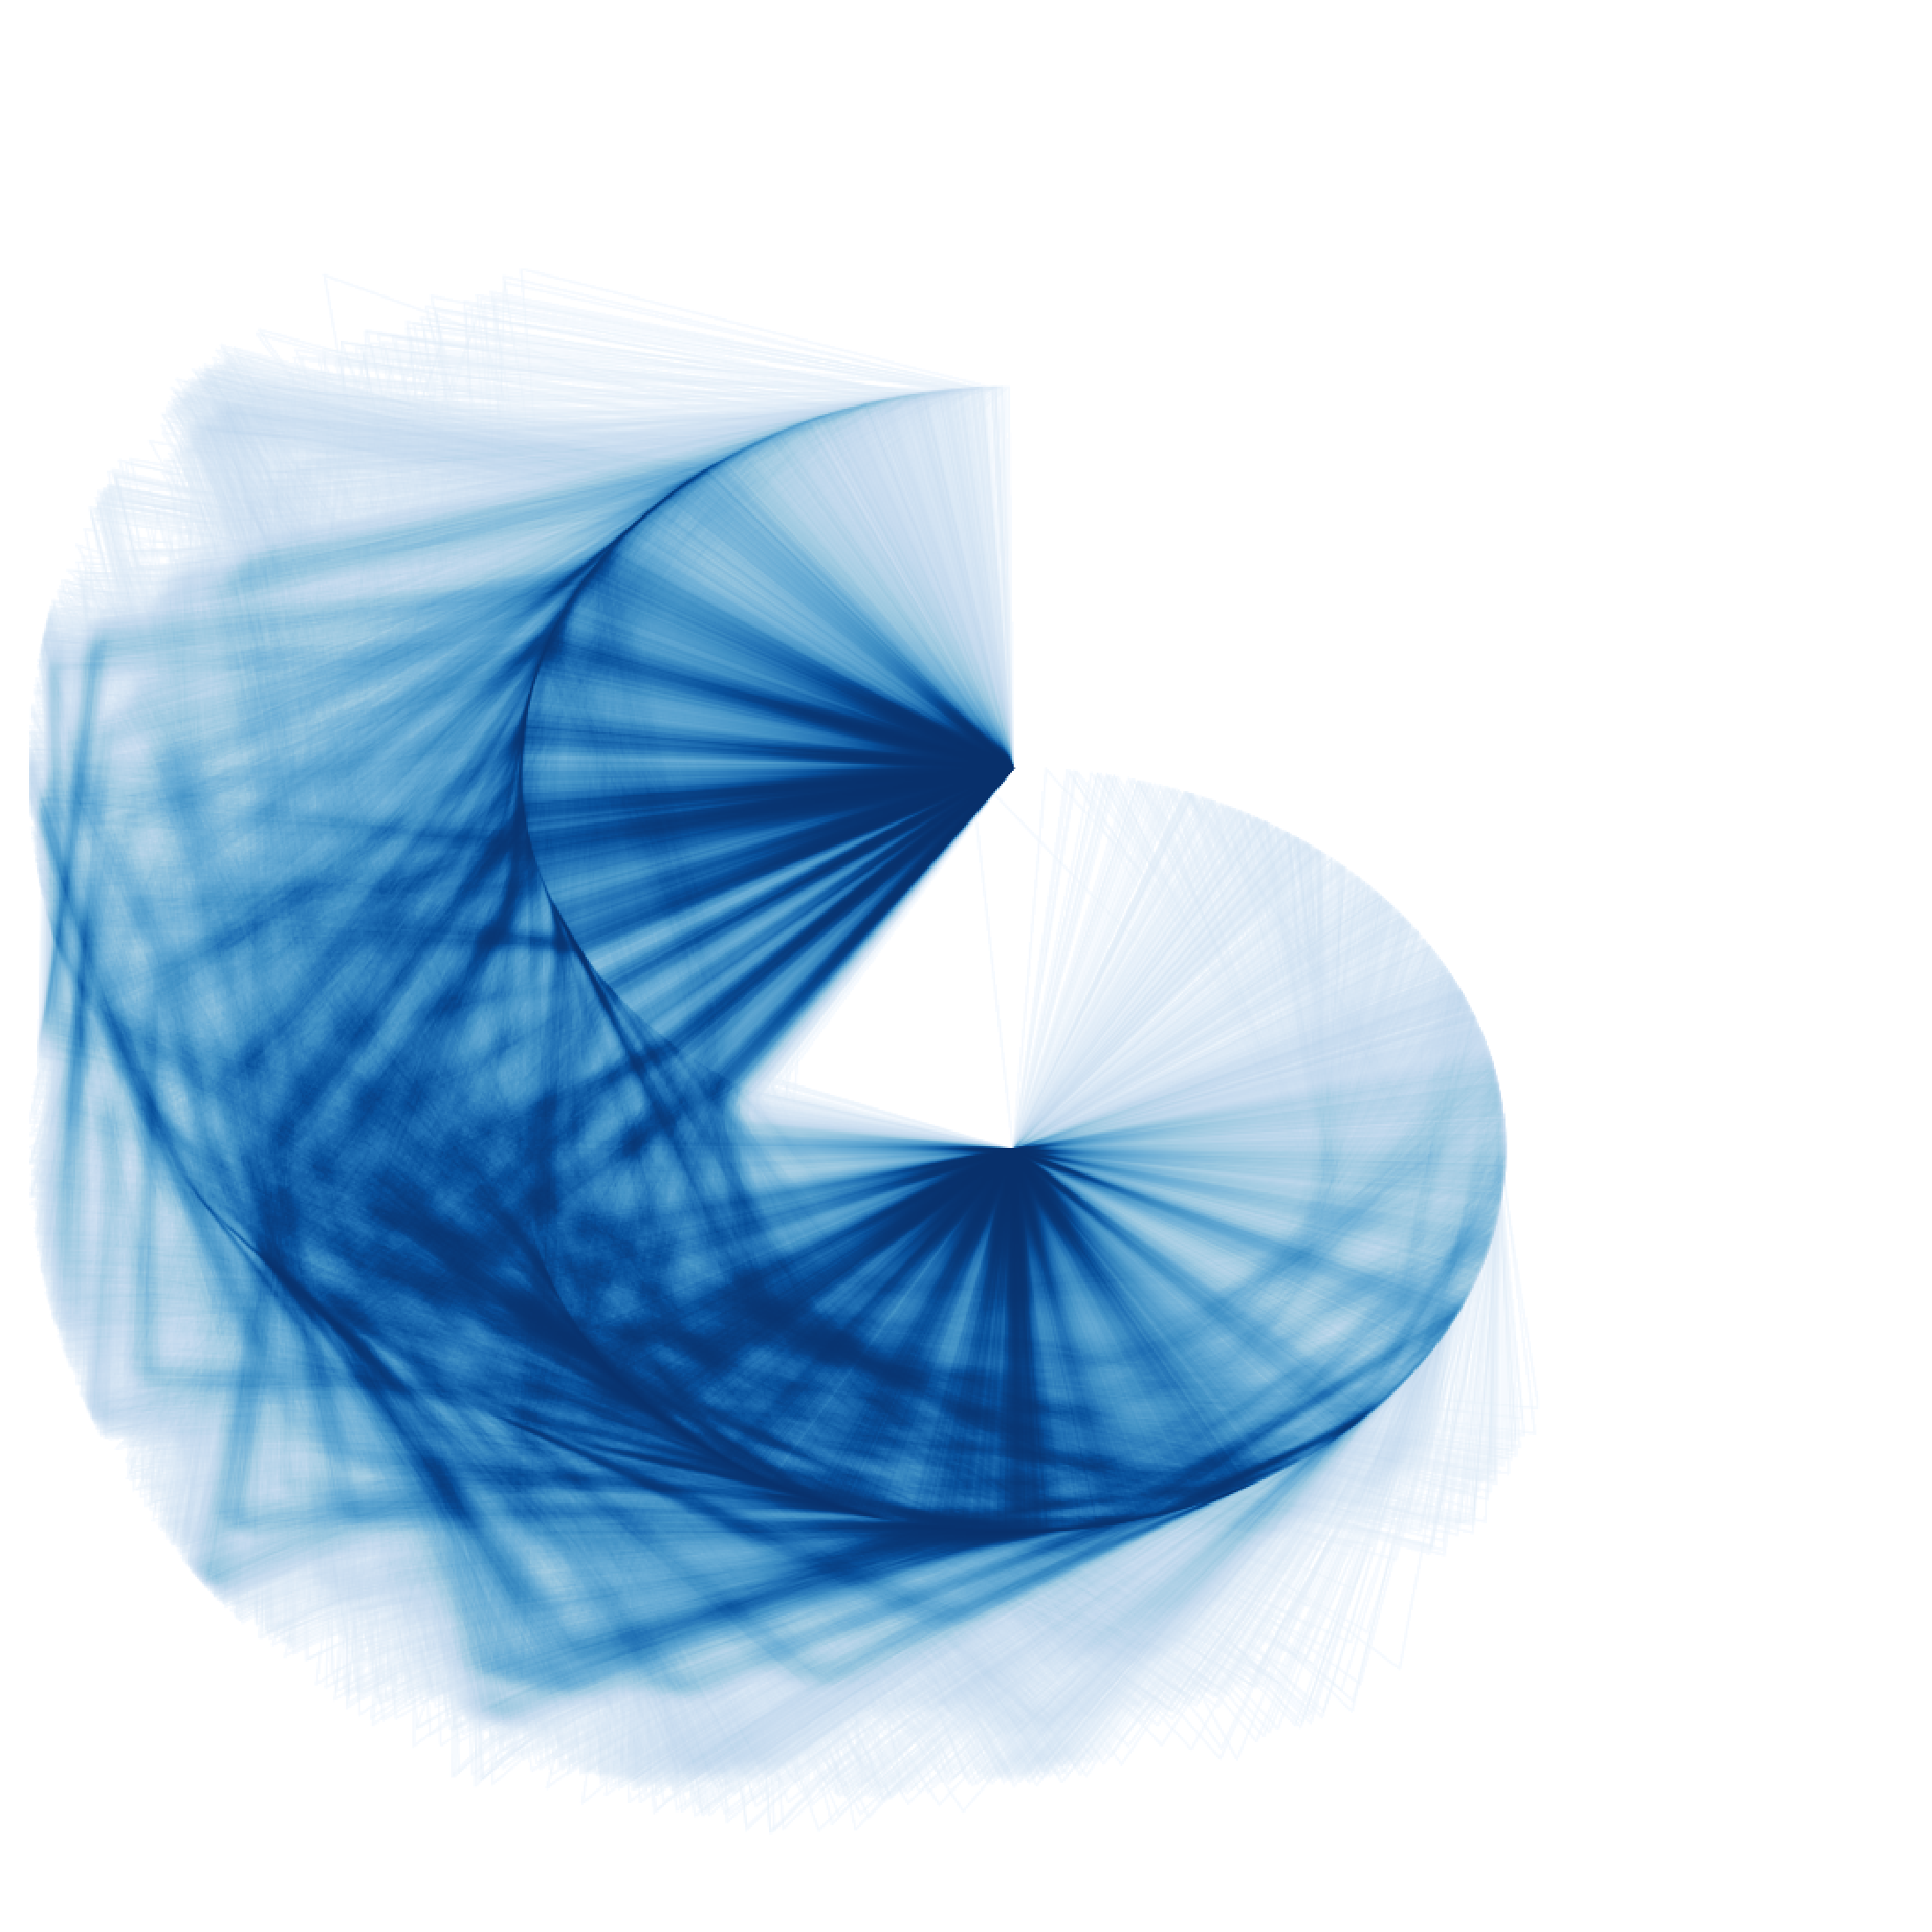
\includegraphics[width=\linewidth]{images/constraind_diffusion_rejection/loops_planar_data.pdf}
		\caption{Data distribution.}
		\label{fig:loop_data}
	\end{subfigure}
	\hfill
	\begin{subfigure}[t]{0.23\textwidth}
		\centering
		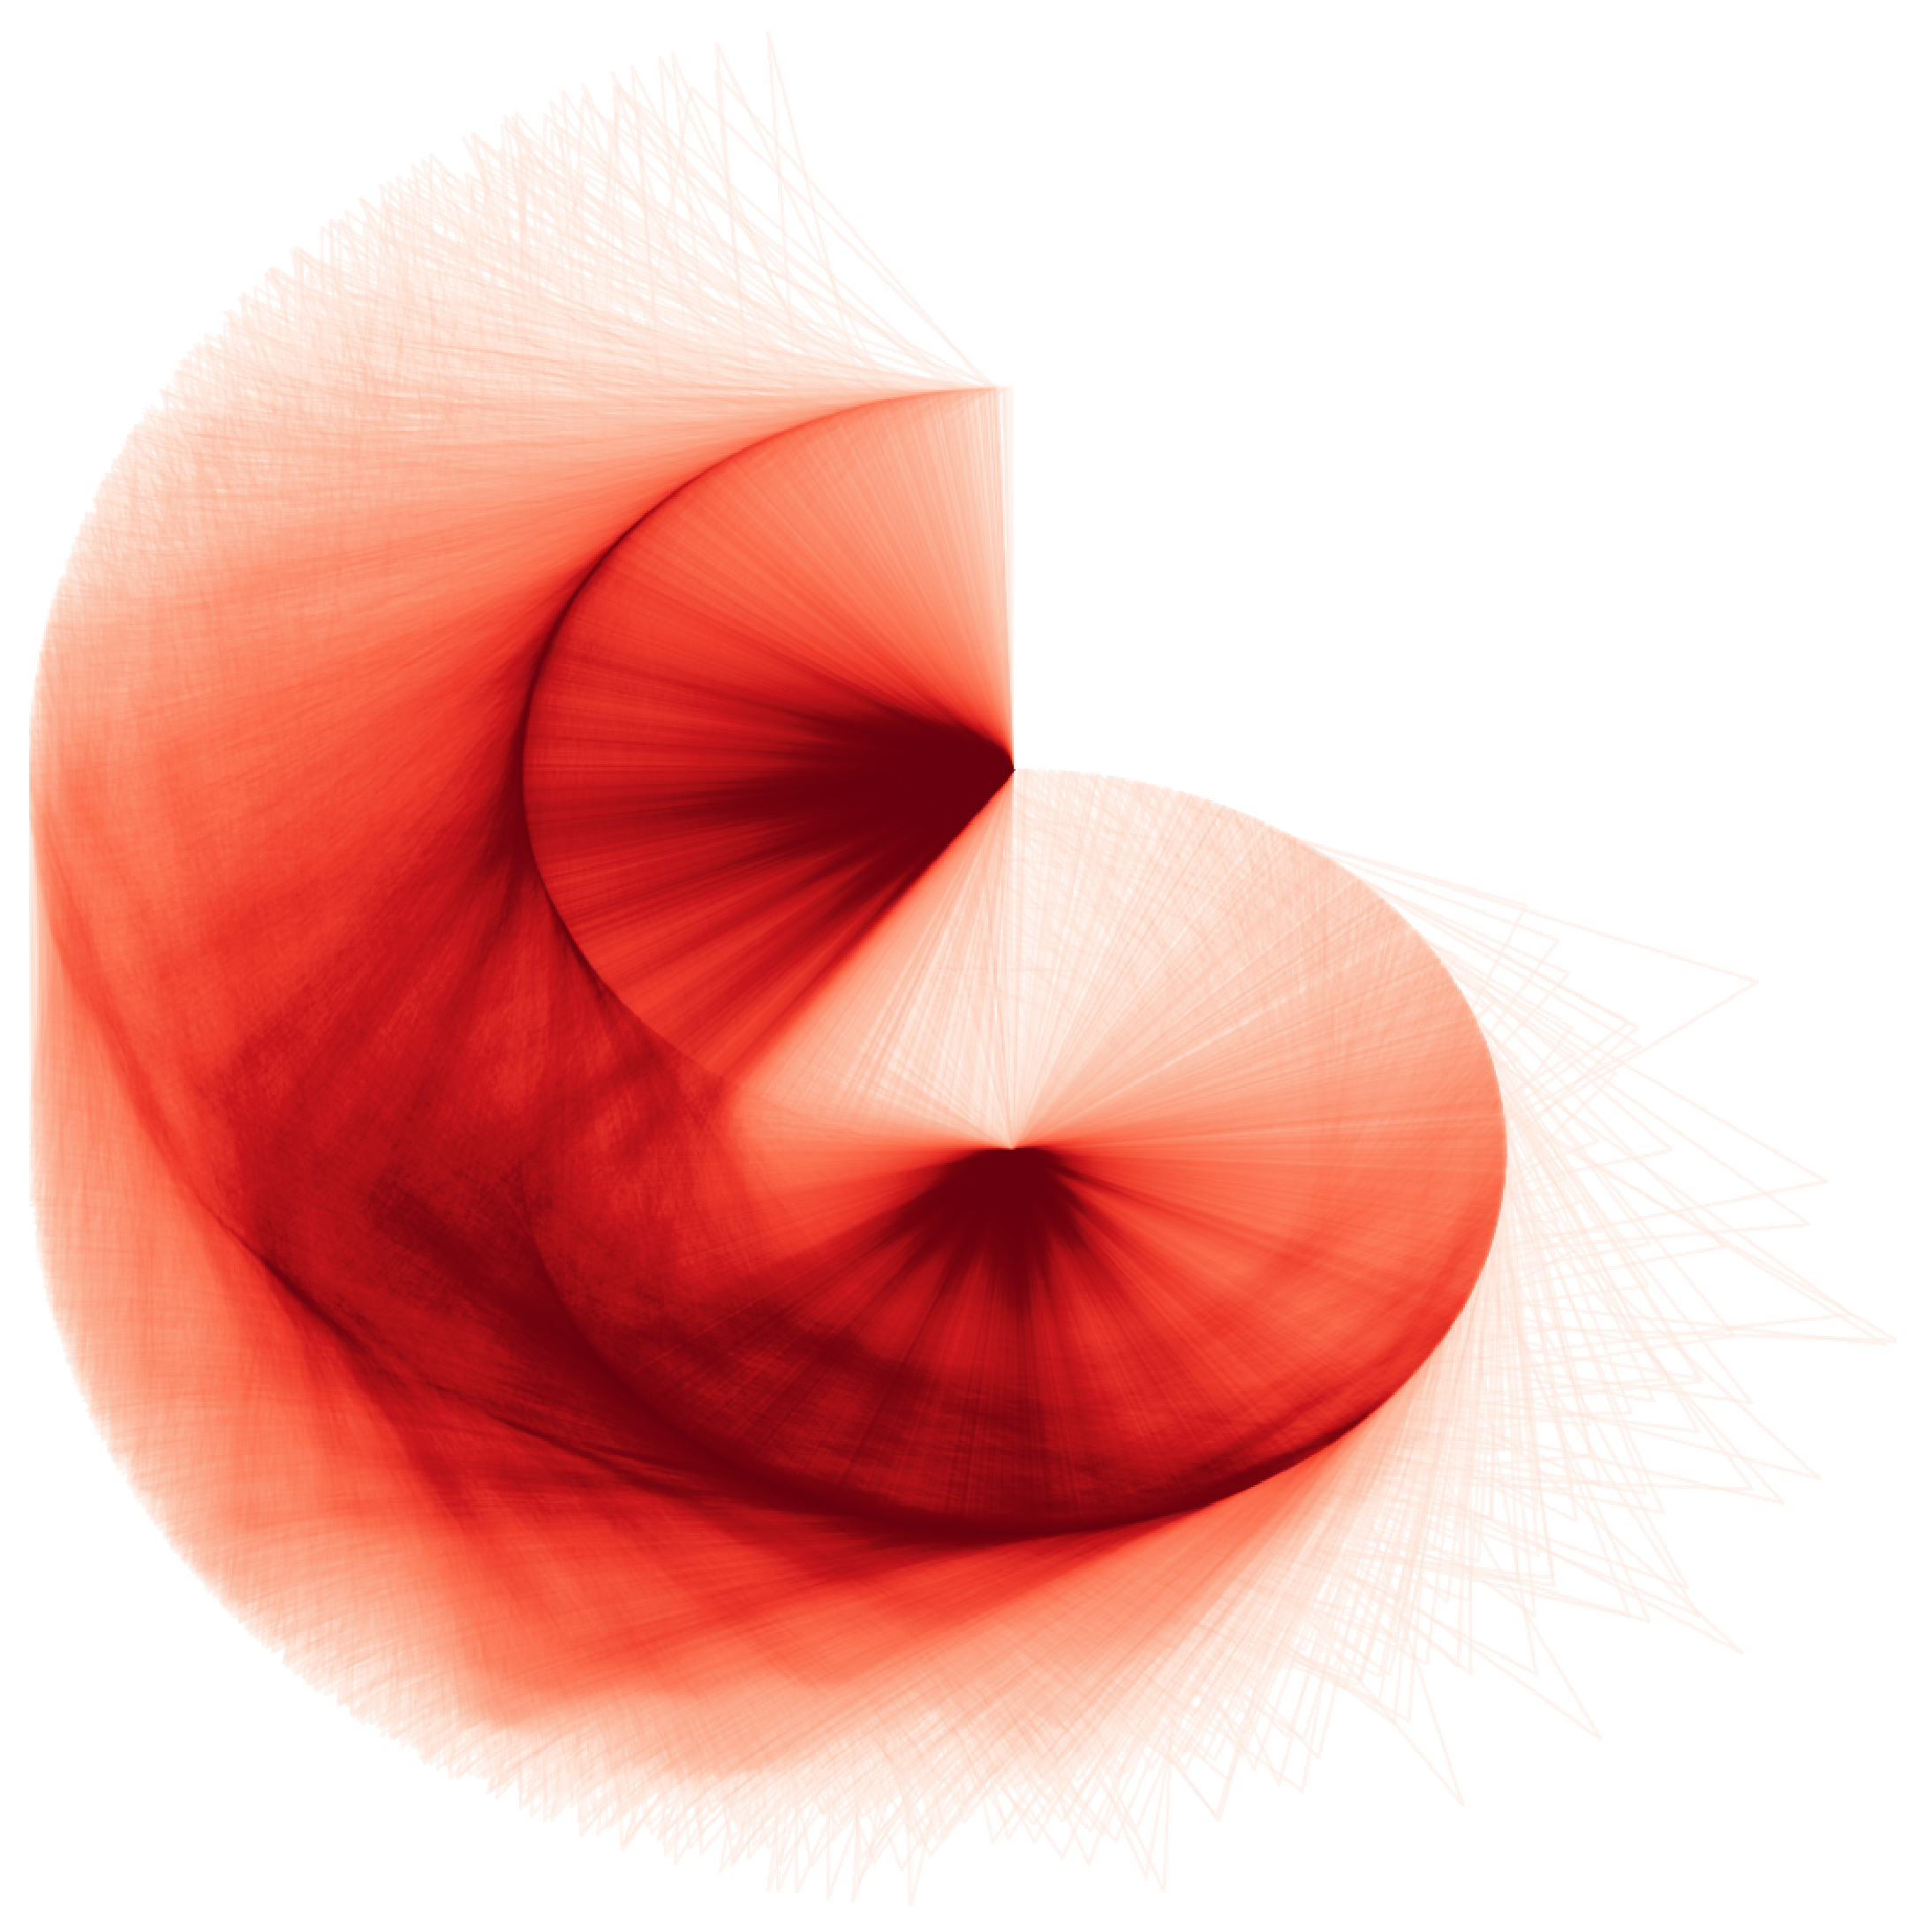
\includegraphics[width=\linewidth]{images/constraind_diffusion_rejection/loops_planar_rejection.pdf}
		\caption{Metropolis samples.}
		\label{fig:loop_rejection}
	\end{subfigure}
	\hfill
	\begin{subfigure}[t]{0.23\textwidth}
		\centering
		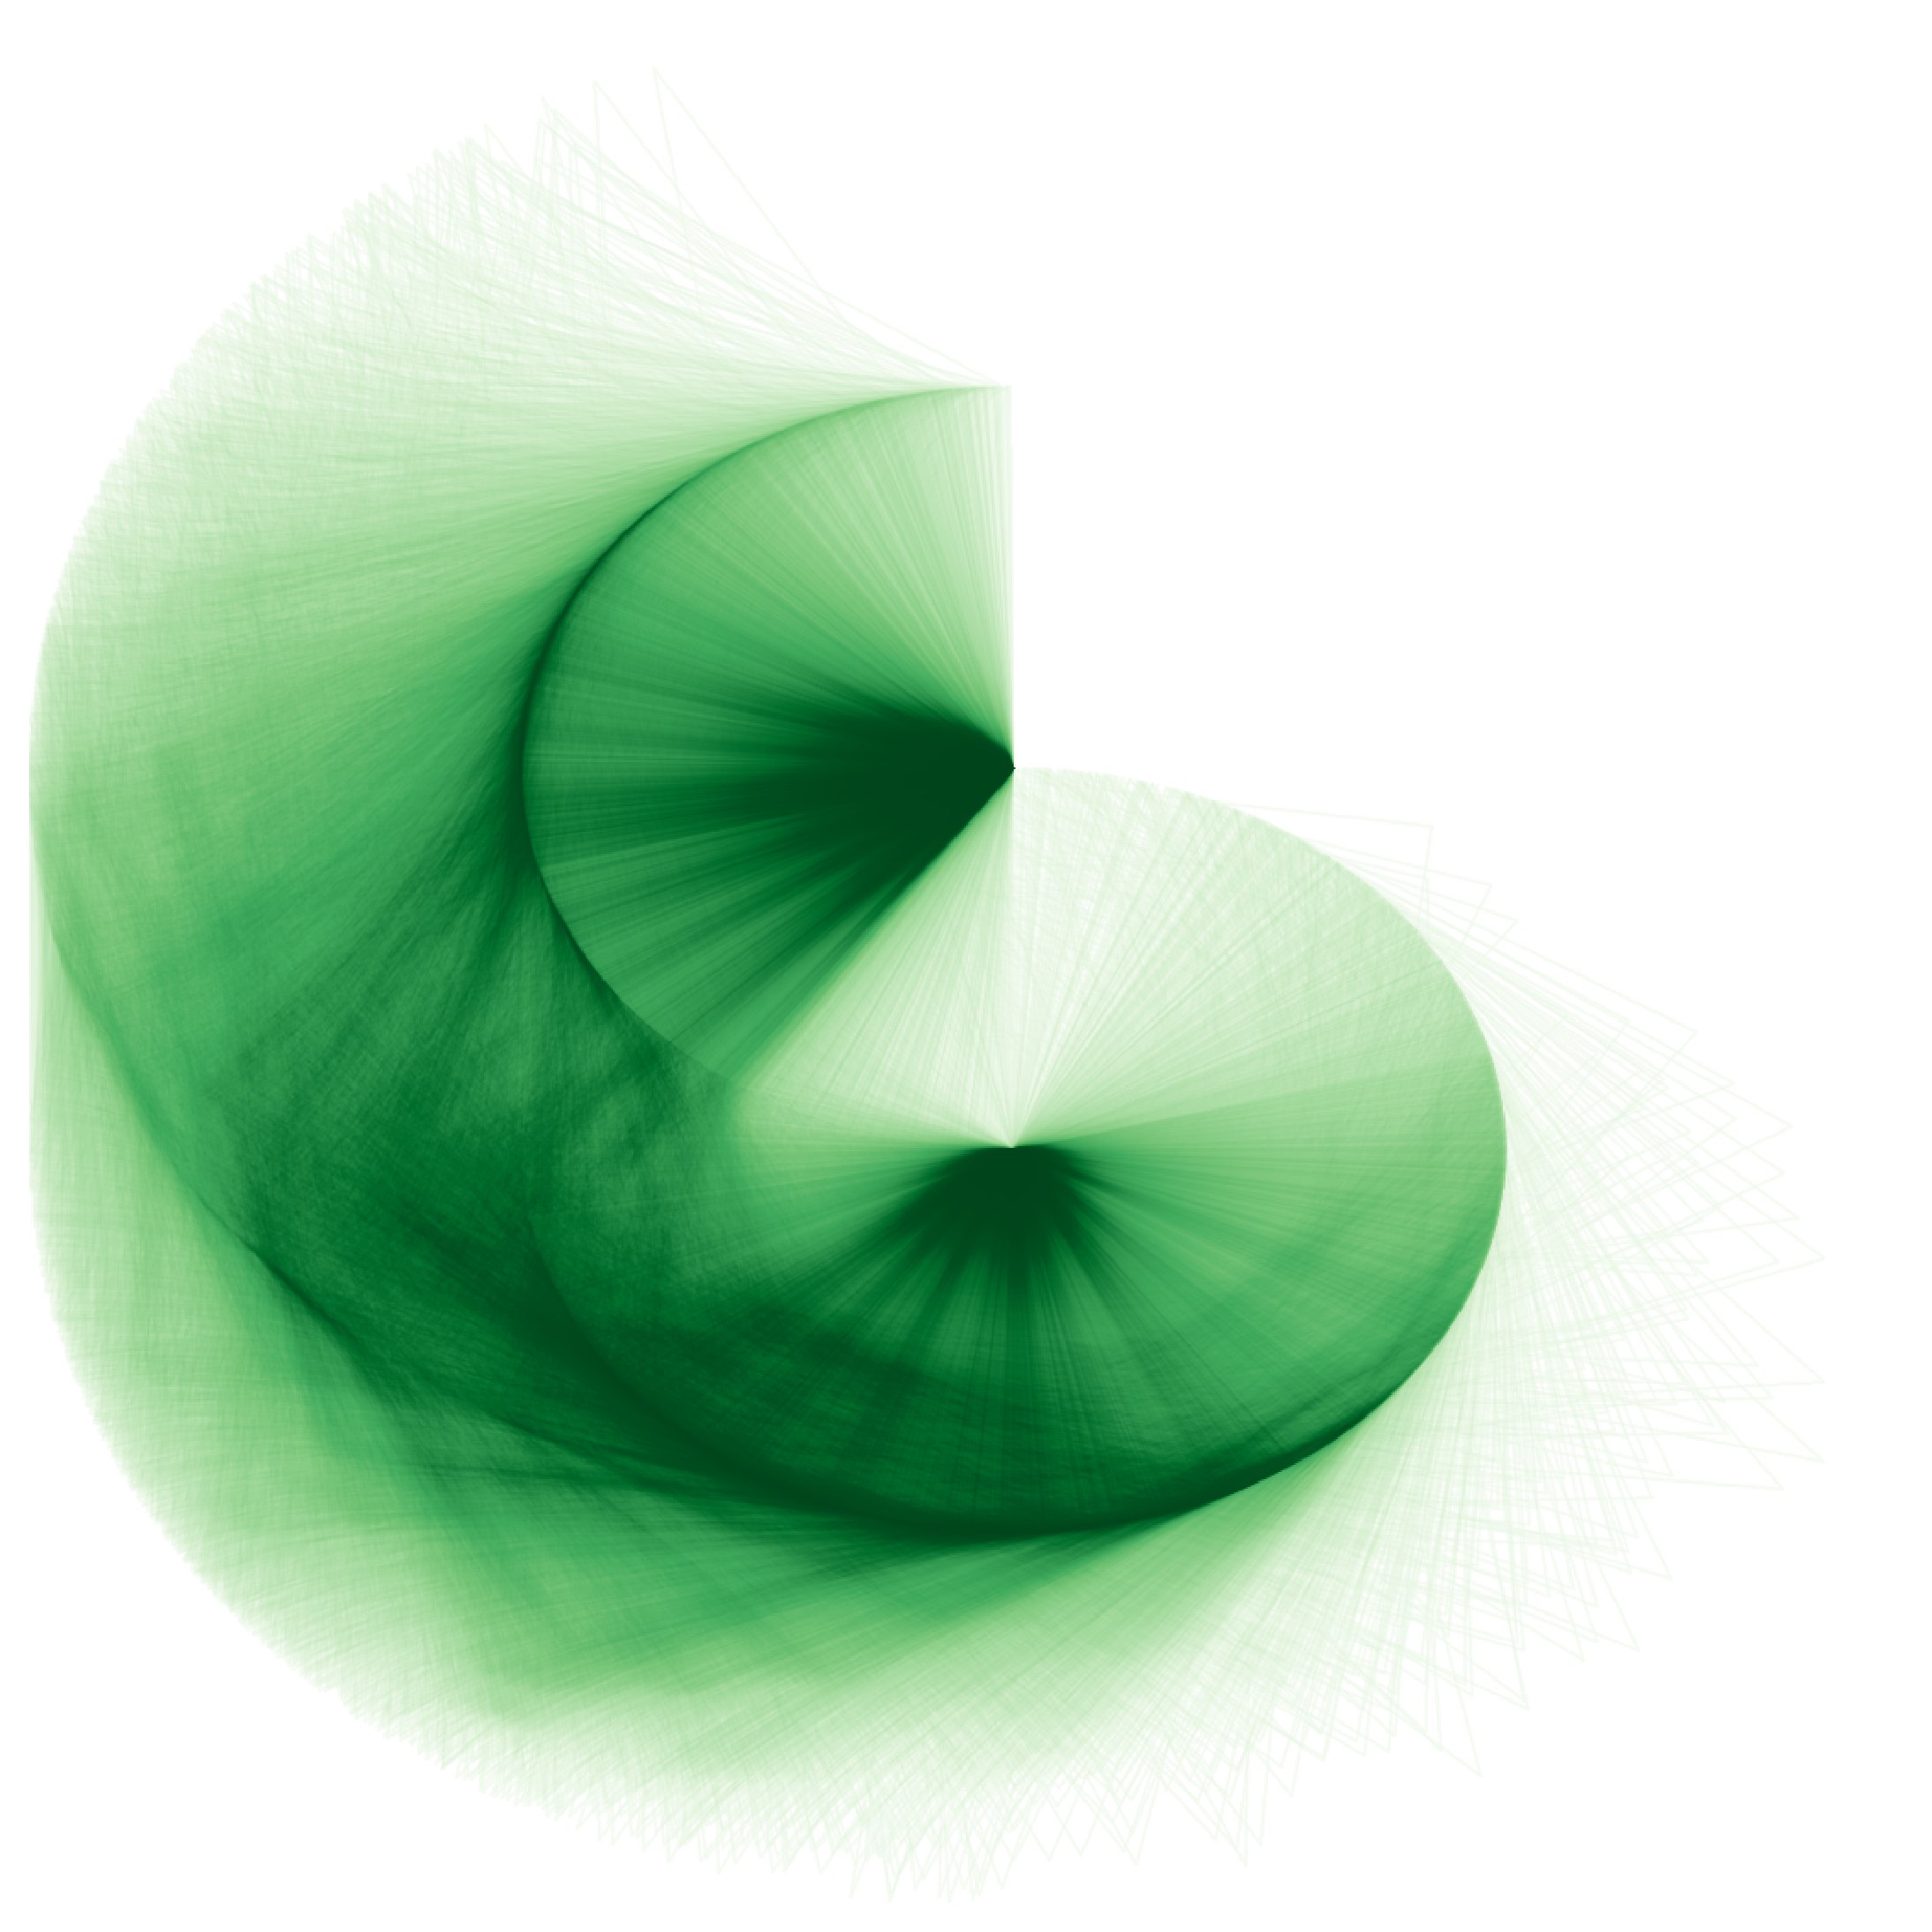
\includegraphics[width=\linewidth]{images/constraind_diffusion_rejection/loops_planar_reflected.pdf}
		\caption{Reflected samples.}
		\label{fig:loop_reflected}
	\end{subfigure}
	\hfill
	\begin{subfigure}[t]{0.23\textwidth}
		\centering
		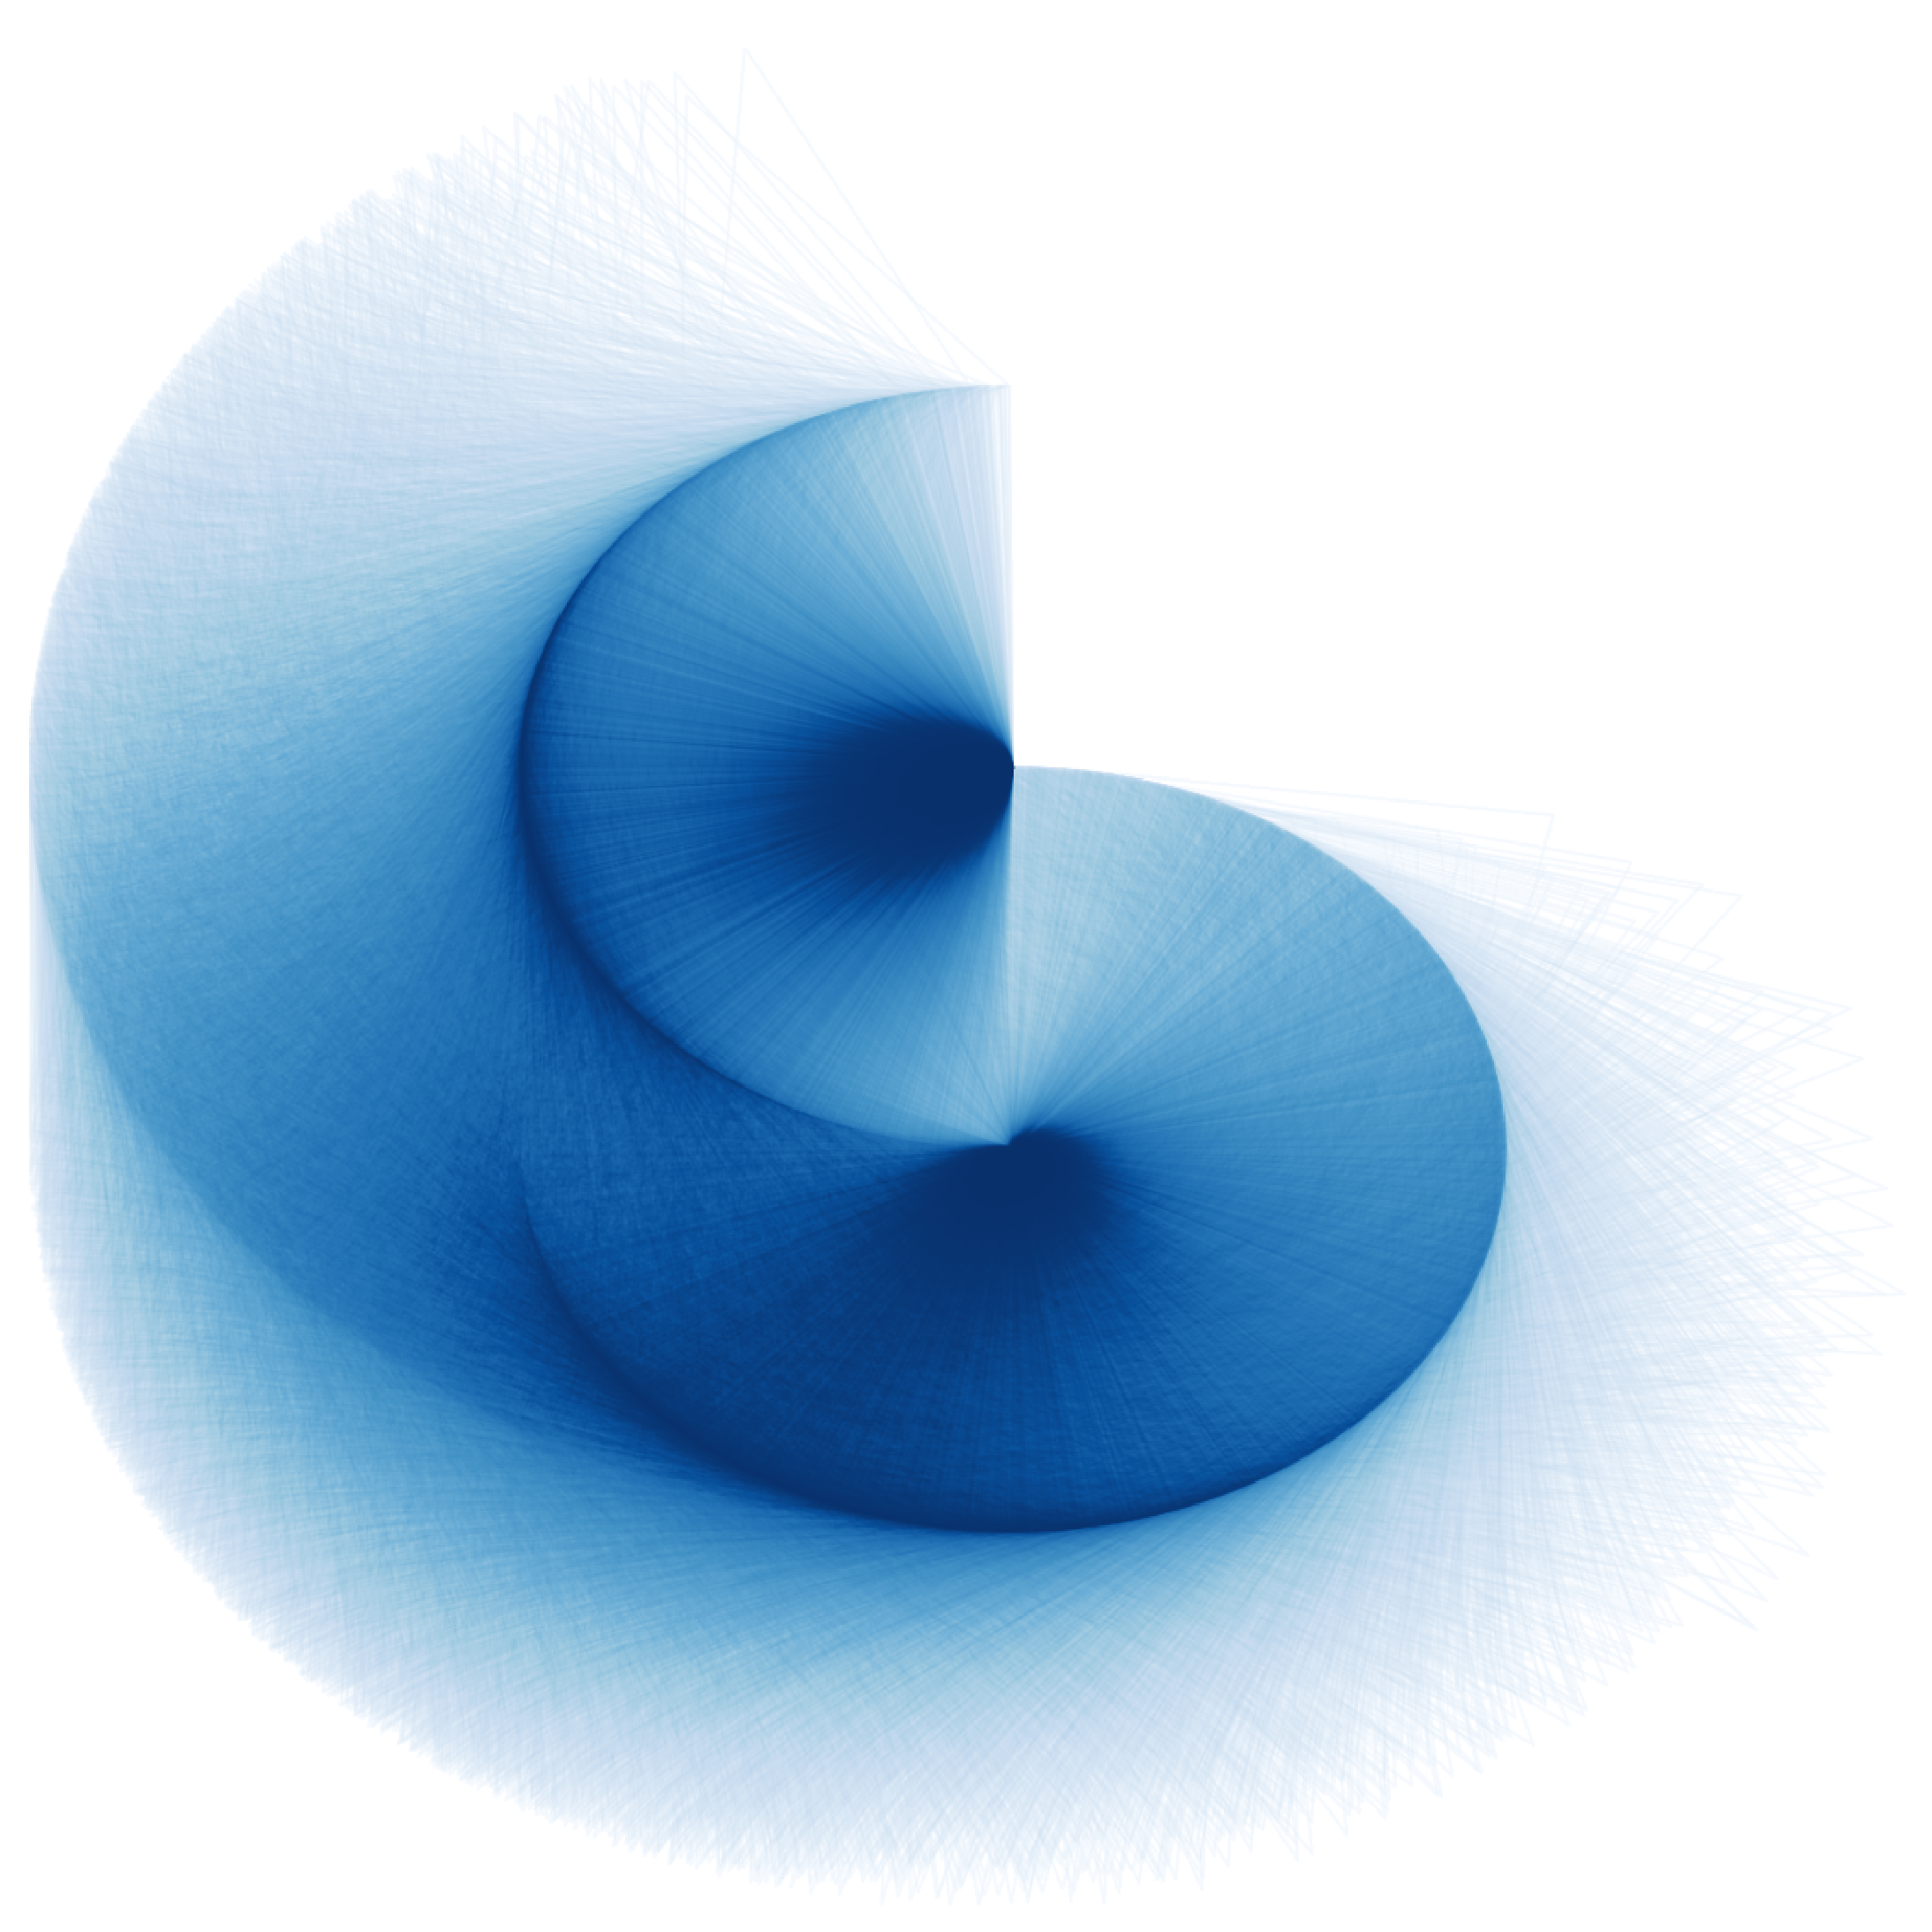
\includegraphics[width=\linewidth]{images/constraind_diffusion_rejection/loops_planar_uniform.pdf}
		\caption{Uniform distribution.}
		\label{fig:loop_uniform}
	\end{subfigure}
	\caption{A qualitative comparison of $10^5$ samples from the data distribution,  our Metropolis diffusion model, a reflected diffusion model and the uniform distribution for the constrained conformational modelling of cyclic peptide backbones.
		For visual clarity, the figures only show the constrained planar projections encoded by \(\mathbb{P}\subset\R^3\).
	}
	\label{fig:loop}
\end{figure}

\paragraph{Conformational modelling of protein backbones.}
Modelling the conformational ensembles of proteins is a data-scarce problem with a range of important applications in biotechnology and drug discovery \parencite{lane2023protein}.
In many practical settings, it may often be unnecessary to model the structural ensembles of an entire protein, as researchers are primarily interested in specific functional sites that are embedded in a structurally conserved scaffold \parencite{huang2016coming}.
Modelling the conformational ensembles of such substructural elements requires positional constraints on their endpoints to ensure that they can be accommodated by the remaining protein.
Using the parametrisation and dataset presented in \cite{fishman2023diffusion}, we formulate the problem of modelling the backbone conformations of a cyclic peptide of length $N=6$ as learning a distribution over the product of a polytope \(\mathbb{P}\subset\R^{3}\) and the hypertorus \(\mathbb{T}^{4}\).

\begin{table}[H]
	\caption{
		Log-likelihood ($\uparrow$) of a held-out test set for the robotics and protein applications.
		Means and standard deviations are computed over 3 different runs.
		Training time in hours is listed in parentheses.
	}
	\label{tab:real_world_data}
	\centering

	\vspace{1em}
	\begin{tabular}{llll}
		\toprule
		Dataset  & Domain                                      & {Reflected \emph{(hours)}}     & {Metropolis \emph{(hours)}}             \\
		\midrule
		Robotics & \(\c{S}_{++}^2\times\R^2\)                  & $8.39 \pm{.06}$ \emph{(9.52)}  & $\mathbf{9.13 \pm{.03}}$ \emph{(1.36)}  \\
		Proteins & \(\mathbb{P}\subset\R^3\times\mathbb{T}^4\) & $15.20\pm{.06}$ \emph{(24.80)} & $\mathbf{15.33 \pm{.02}}$ \emph{(3.12)} \\
		\bottomrule
	\end{tabular}
\end{table}

We quantify the empirical performance of different methods by evaluating the log-likelihood of a held-out test set and present the resulting performance metrics in~\Cref{tab:real_world_data}.

Again, we find that our Metropolis model outperforms the reflected approach by a statistically significant margin while training 7-8 times as fast.
Qualitative visual comparisons of samples from the true distribution, the trained diffusion models and the uniform distribution are presented in~\Cref{fig:robotic_arm,fig:loop}, with full univariate marginal and pairwise bivariate correlation plots postponed to~\Cref{sec:app_robotic_arms_spd,sec:app_loop_pairplots}.

\subsection{Modelling geospatial data within non-convex country borders}
\label{sec:exp_wildfires}

Motivated by the strong empirical performance of our approach on tasks with challenging convex constraints, we investigate its ability to approximate distributions whose support is restricted to manifolds with highly non-convex boundaries---a setting that is intractable with existing approaches.
To this end, we derived a geospatial dataset based on wildfire incidence rates within the continental United States (see~\Cref{app_sec:wildfire_data} for full details) and trained a Metropolis diffusion model constrained by the corresponding country borders on the sphere $\c{S}^2$.
A qualitative visual comparison of samples from the true distribution, our model, and the uniform distribution is presented in~\Cref{fig:wildfire_data_dist,fig:wildfire_rejection_dist,fig:wildfire_uniform_dist}, demonstrating that our approach is able to successfully model challenging multimodal and sparse distributions on constrained manifolds with highly non-convex boundaries.

\begin{figure}[t]
	\centering
	\begin{subfigure}[t]{0.28\textwidth}
		\centering
		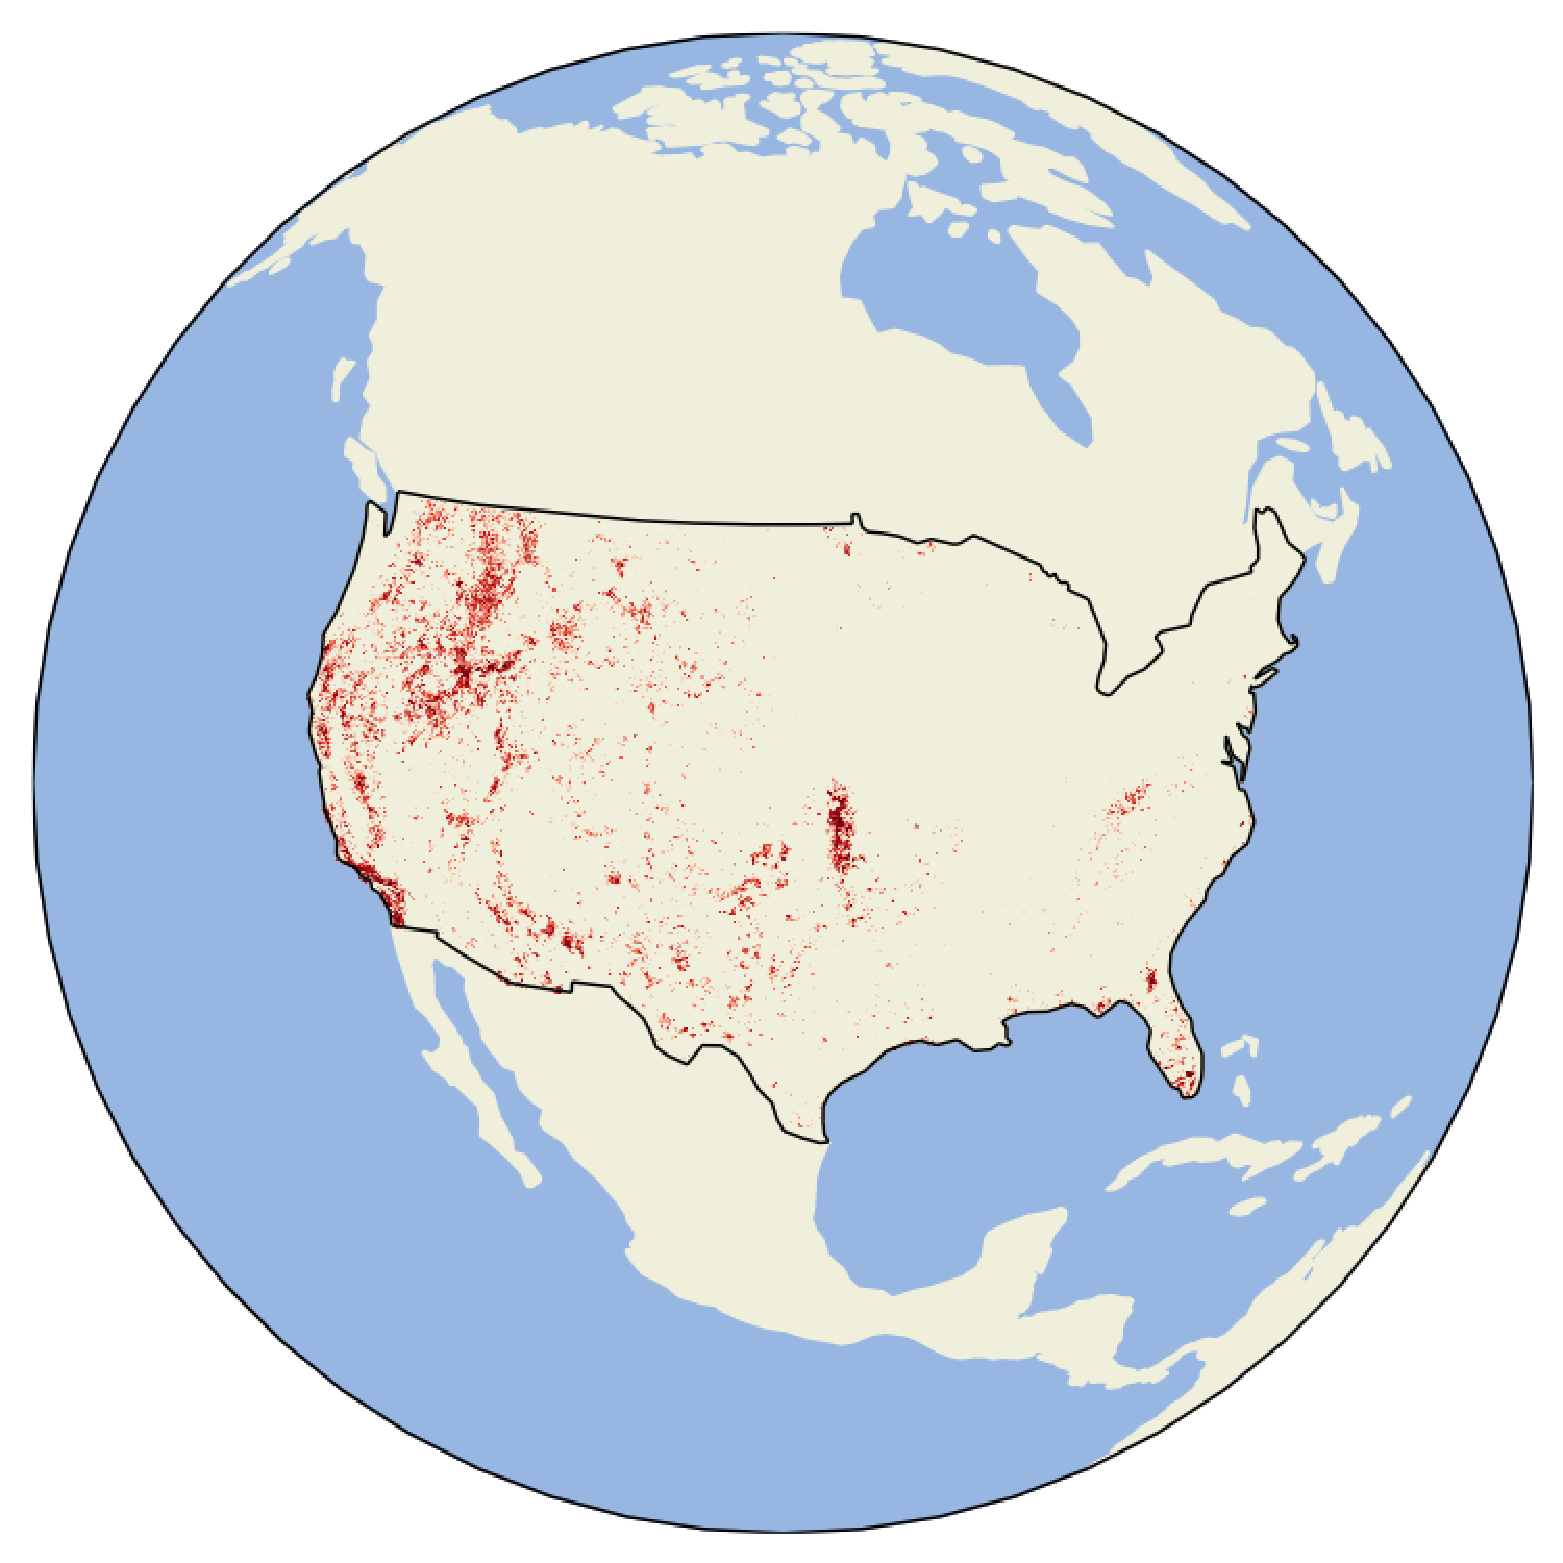
\includegraphics[width=\linewidth]{images/constraind_diffusion_rejection/wildfire_data_dist.pdf}
		\caption{Data distribution.}
		\label{fig:wildfire_data_dist}
	\end{subfigure}
	\hfill
	\begin{subfigure}[t]{0.28\textwidth}
		\centering
		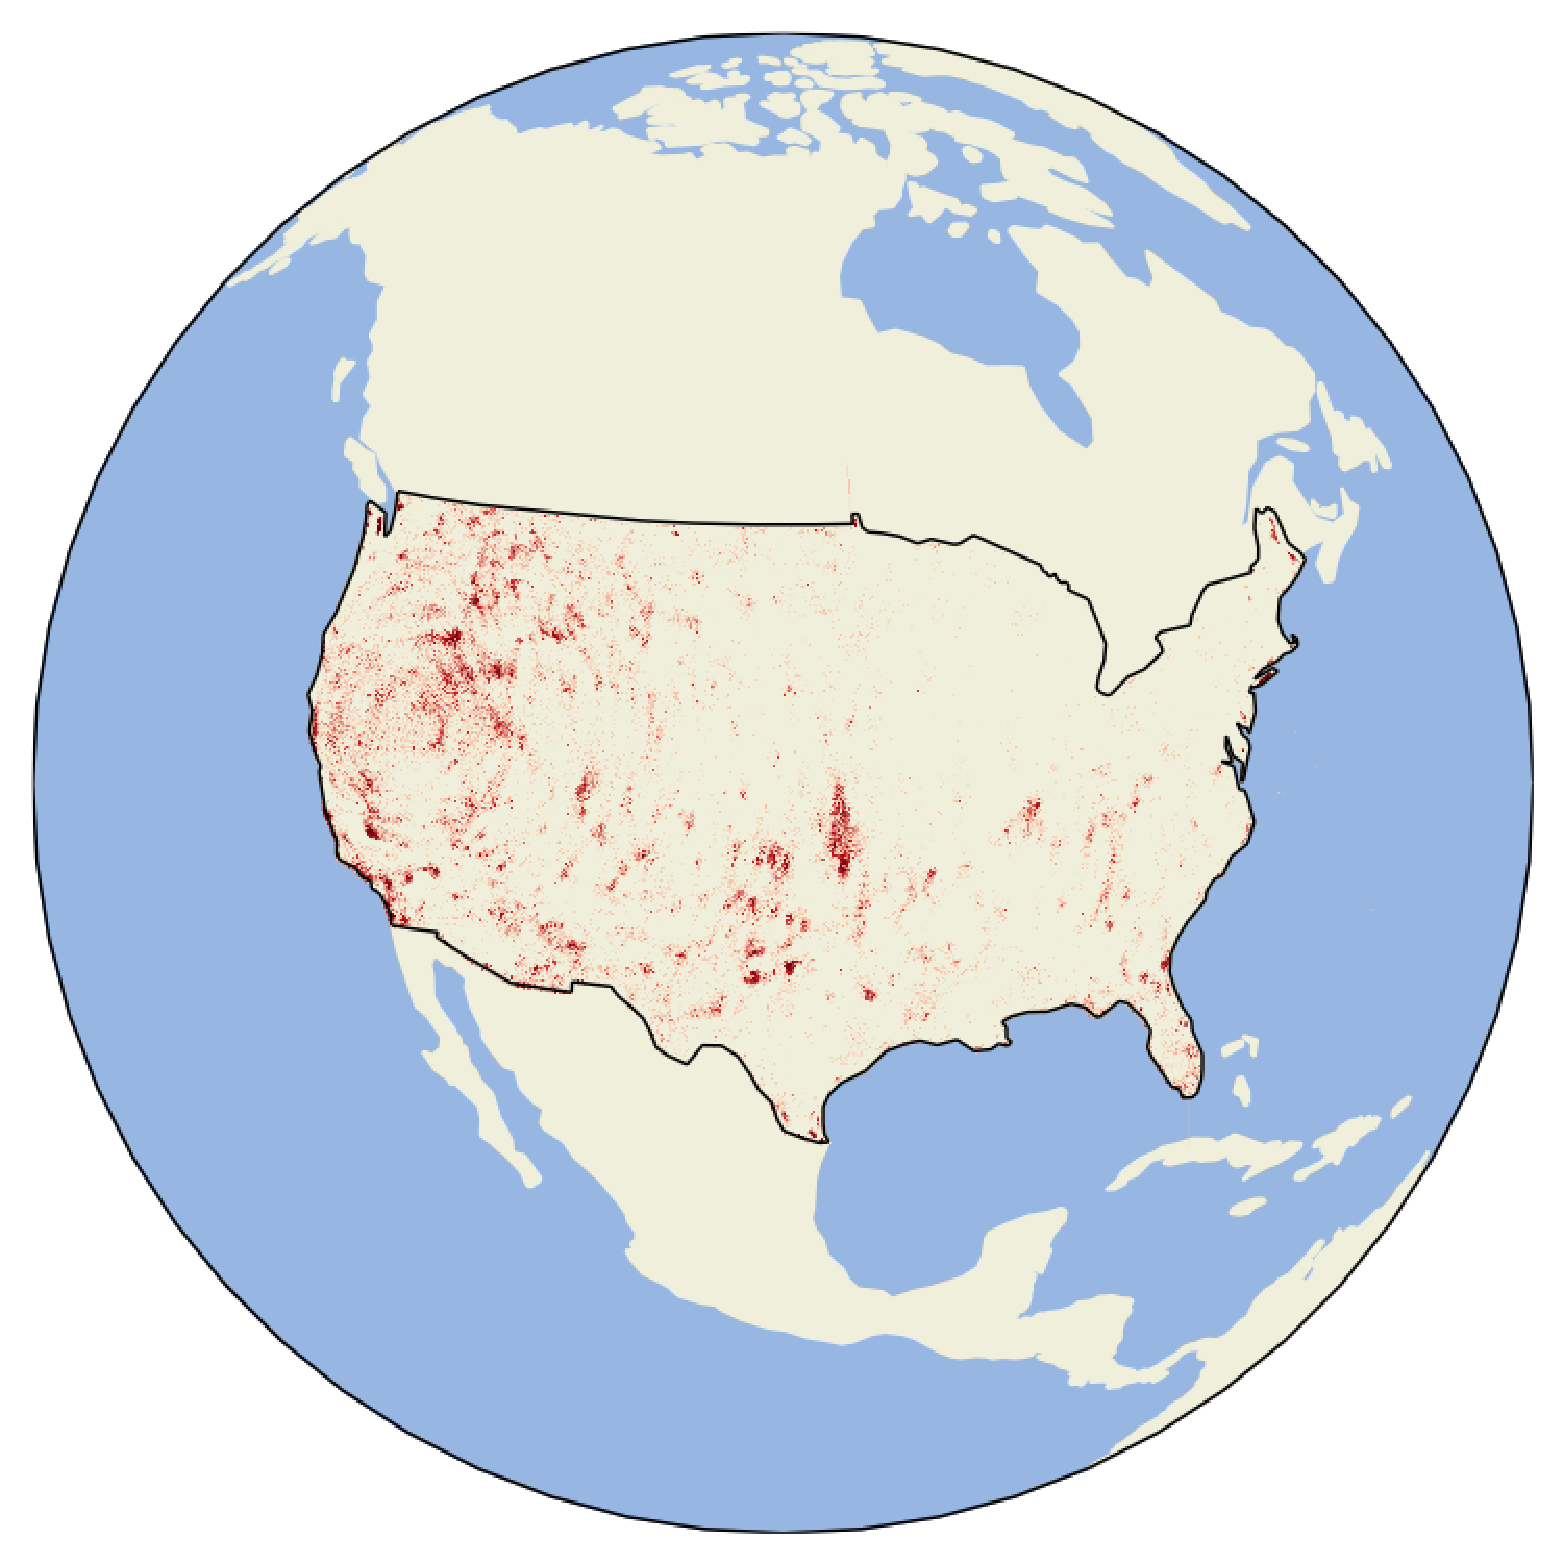
\includegraphics[width=\linewidth]{images/constraind_diffusion_rejection/wildfire_rejection_dist.pdf}
		\caption{Metropolis samples.}
		\label{fig:wildfire_rejection_dist}
	\end{subfigure}
	\hfill
	\begin{subfigure}[t]{0.28\textwidth}
		\centering
		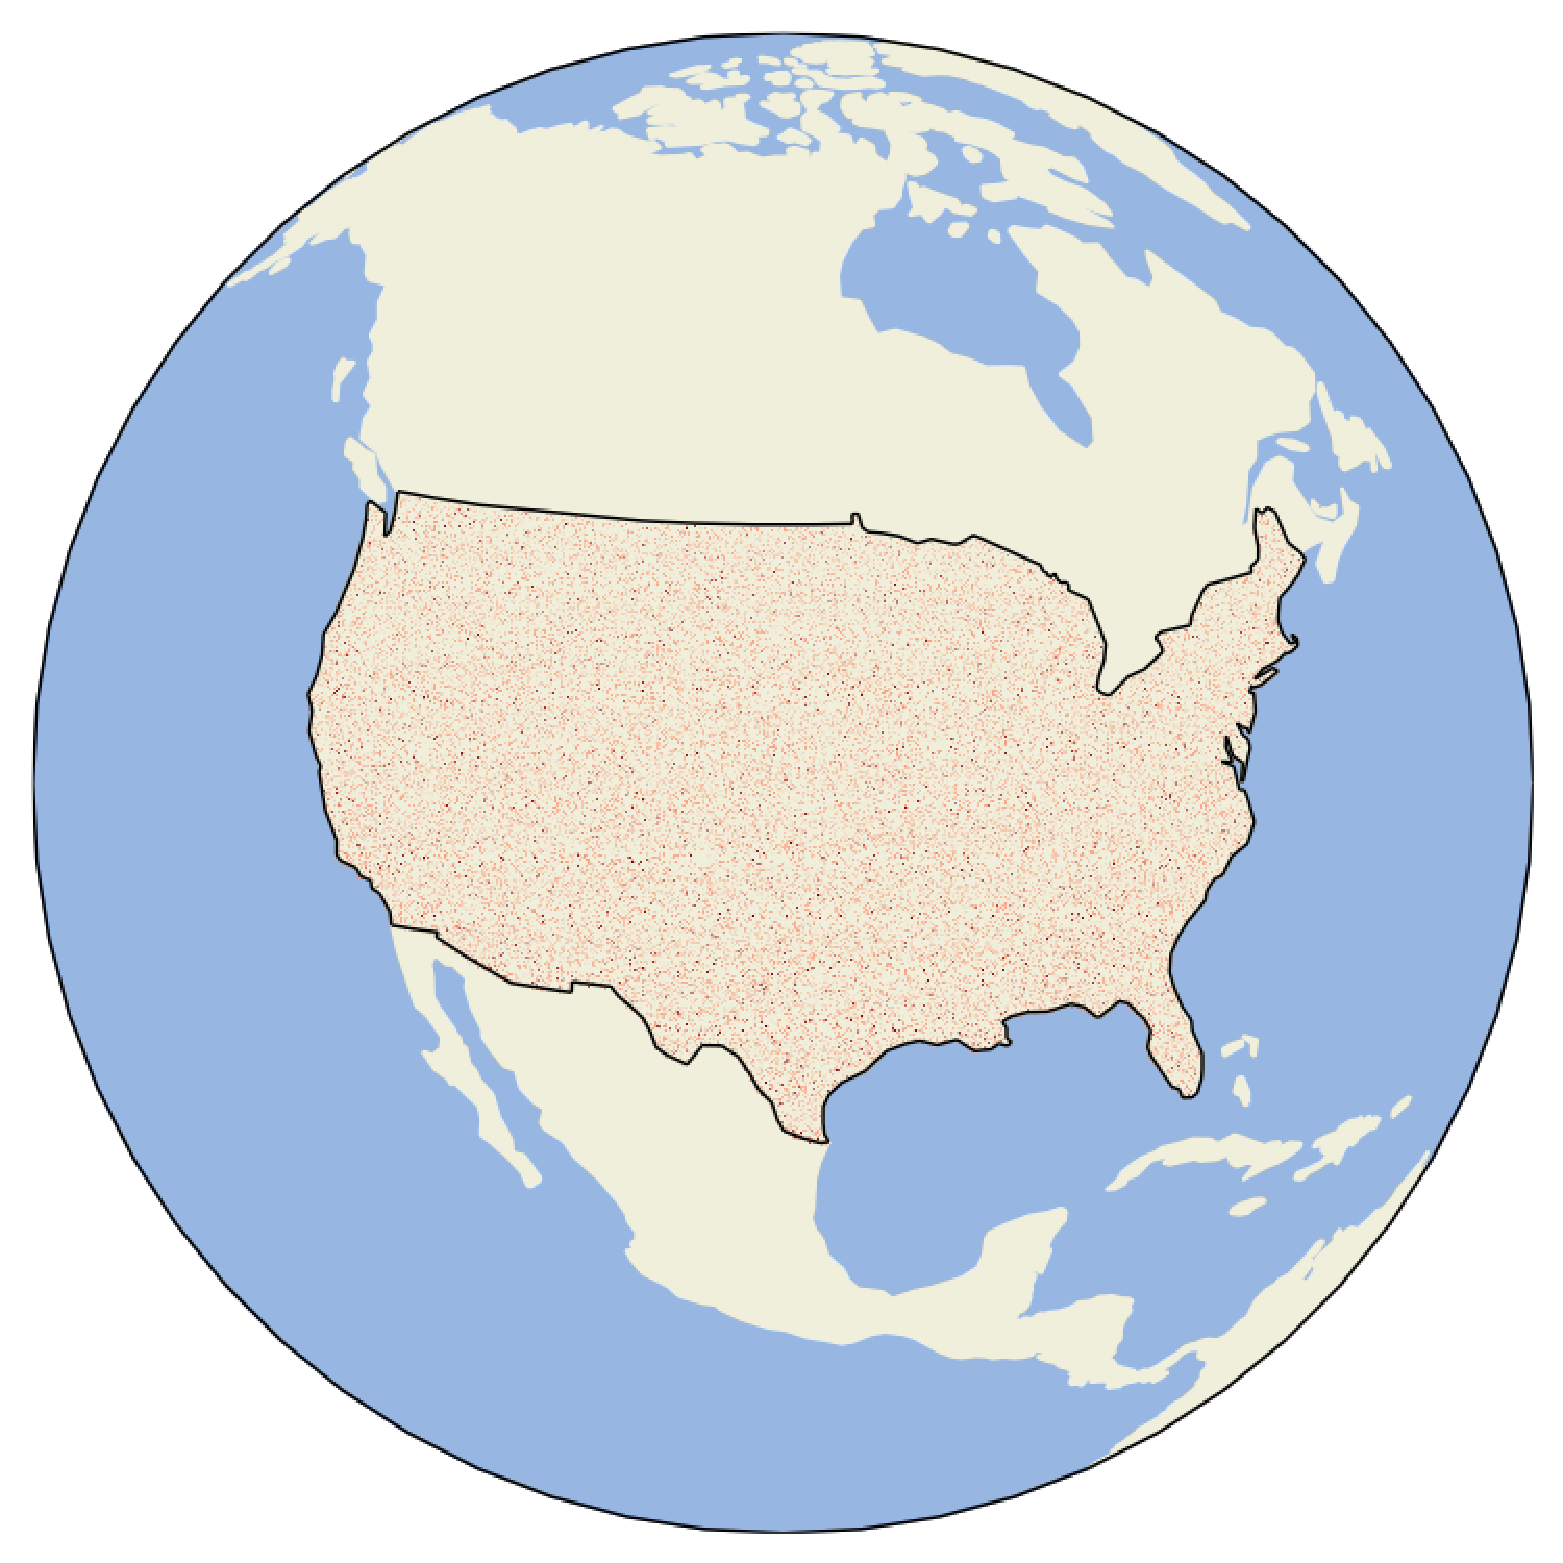
\includegraphics[width=\linewidth]{images/constraind_diffusion_rejection/wildfire_uniform_dist.pdf}
		\caption{Uniform distribution.}
		\label{fig:wildfire_uniform_dist}
	\end{subfigure}
	\caption{Orthographic projection of $10^5$ samples from (a) the data distribution, (b) our Metropolis diffusion model, and (c) the uniform distribution, for geospatial data (wildfire incidence rates) within a non-convex boundary (the continental United States).
		The projections are aligned with the geometric centre of the boundary and zoomed in ten-fold for visual clarity.
	}
	\label{fig:wildfire_headline_plot}
\end{figure}

\section{Conclusion}

Accurately modelling distributions on constrained Riemannian manifolds is a challenging problem with a range of impactful practical applications.
In this work, we have proposed a mathematically principled and computationally scalable extension of the existing diffusion model methodology to this setting.
Based on a \emph{Metropolisation} of random walks in Euclidean spaces and on Riemannian manifolds, we have shown that our approach corresponds to a valid discretisation of the reflected Brownian motion, justifying its use in diffusion models.
To demonstrate the practical utility of our method, we have performed an extensive empirical evaluation, showing that it outperforms existing constrained diffusion models on a range of synthetic and real-world tasks defined on manifolds with convex boundaries, including applications from robotics and protein design.
Leveraging the flexibility and simplicity of our method, we have also demonstrated that it extends beyond convex constraints and is able to successfully model distributions on manifolds with highly non-convex boundaries.

While we found our method to perform well across the synthetic and real-world applications we considered, we expect it to perform poorly on certain constraint geometries.
For instance, the current implementation relies on an isotropic noise distribution which could impede its performance on exceedingly narrow constraint geometries, even with correspondingly small step sizes.
In this context, an important direction of future research would be to investigate whether we can instead sample from more suitable distributions, e.g. a Dikin ellipsoid, while maintaining the simplicity and efficiency of the Metropolis approach.
More general topics of future work include the derivation of quantitative weak and mean square errors of our proposed discretisation scheme, as well as its application to more semantic constraints, for example with the objective of imposing sparsity in a basis or fixing the colour or style of an image.
